% !TEX program = xelatex
\documentclass[11pt,a4paper]{article}

\usepackage[a4paper,top=2cm,bottom=2.2cm,left=2.2cm,right=2.2cm]{geometry}
\usepackage{fontspec}
\usepackage{polyglossia}
\setdefaultlanguage{vietnamese}
\setotherlanguage{english}
\setmainfont{Times New Roman}
\setmonofont{Consolas}[Scale=0.92]

\usepackage{amsmath, amssymb}
\usepackage{graphicx}
\usepackage{xcolor}
\usepackage{colortbl}
\usepackage{booktabs}
\usepackage{tabularx}
\usepackage{array}
\usepackage{enumitem}
\usepackage{tcolorbox}
\usepackage{listings}
\usepackage{caption}
\usepackage{titlesec}
\usepackage[hidelinks,colorlinks=true,linkcolor=blue!60!black,urlcolor=blue!60!black]{hyperref}

% ----- colors
\definecolor{usthblue}{HTML}{0054A6}
\definecolor{darkblue}{HTML}{003366}
\definecolor{softgray}{HTML}{F5F6F8}
\definecolor{boxborder}{HTML}{D8E0EA}
\definecolor{kwcol}{HTML}{0033CC}
\definecolor{strcol}{HTML}{B30000}
\definecolor{cmtcol}{HTML}{717171}
\definecolor{numcol}{HTML}{8E5816}
\definecolor{egbox}{HTML}{FFF8E6}
\definecolor{egbord}{HTML}{E5C97A}

% ----- listings
\lstdefinestyle{py}{
  language=Python,
  basicstyle=\ttfamily\footnotesize,
  keywordstyle=\color{kwcol}\bfseries,
  stringstyle=\color{strcol},
  commentstyle=\color{cmtcol}\itshape,
  numberstyle=\tiny\color{numcol},
  numbers=left,
  numbersep=8pt,
  showstringspaces=false,
  breaklines=true,
  breakatwhitespace=true,
  frame=single,
  rulecolor=\color{boxborder},
  backgroundcolor=\color{softgray},
  framerule=0.4pt,
  xleftmargin=12pt,
  xrightmargin=4pt,
  aboveskip=8pt,
  belowskip=8pt,
  literate={→}{$\rightarrow$}{1}
           {≥}{$\geq$}{1}
           {≤}{$\leq$}{1}
           {α}{$\alpha$}{1}
           {ε}{$\varepsilon$}{1}
           {λ}{$\lambda$}{1}
           {·}{$\cdot$}{1}
}
\lstset{style=py}

% ----- section styling
\titleformat{\section}{\Large\bfseries\color{usthblue}}{\thesection.}{0.5em}{}
\titleformat{\subsection}{\large\bfseries\color{darkblue}}{\thesubsection.}{0.5em}{}
\titleformat{\subsubsection}{\normalsize\bfseries}{}{0pt}{}
\titlespacing*{\section}{0pt}{16pt}{8pt}
\titlespacing*{\subsection}{0pt}{12pt}{6pt}

% ----- boxes
\newtcolorbox{idea}[1][]{
  colback=blue!4, colframe=usthblue!60, boxrule=0.6pt,
  arc=4pt, left=10pt, right=10pt, top=6pt, bottom=6pt,
  title=#1, fonttitle=\bfseries\color{usthblue}
}
\newtcolorbox{example}[1][Ví dụ]{
  colback=egbox, colframe=egbord, boxrule=0.6pt,
  arc=4pt, left=10pt, right=10pt, top=6pt, bottom=6pt,
  title={\footnotesize #1}, fonttitle=\bfseries\color{black!70},
  before skip=8pt, after skip=8pt
}
\newtcolorbox{note}{
  colback=gray!5, colframe=gray!40, boxrule=0.4pt,
  arc=3pt, left=8pt, right=8pt, top=4pt, bottom=4pt,
  before skip=6pt, after skip=6pt
}

\setlength{\parskip}{6pt}
\setlength{\parindent}{0pt}
\renewcommand{\arraystretch}{1.2}

% ----- title block
\title{
  \vspace{-1.5cm}
  \color{usthblue}\Huge\textbf{Cẩm nang kiến thức đồ án} \\[6pt]
  \color{black!75}\large Phân loại Tổn thương Da bằng Học sâu \\[2pt]
  \normalsize\textit{Từ định nghĩa cơ bản đến chi tiết kỹ thuật}
}
\author{
  Nguyễn Trọng Bách --- 23BI14057 \\[2pt]
  \small Đại học Khoa học và Công nghệ Hà Nội (USTH)
}
\date{}

\begin{document}
\maketitle
\vspace{-1cm}

{\hypersetup{linkcolor=black}\tableofcontents}

\newpage

% ===================================================
\section{Đồ án này là gì --- tóm tắt một trang}
% ===================================================

\textbf{Bài toán.} Cho một ảnh dermoscopy (ảnh soi da bằng kính phóng đại) của một tổn thương trên da, hãy dự đoán nó thuộc một trong \textbf{7 loại}: \texttt{akiec}, \texttt{bcc}, \texttt{bkl}, \texttt{df}, \texttt{mel}, \texttt{nv}, \texttt{vasc}. Trong đó \texttt{mel} (melanoma --- ung thư hắc tố) là lớp nguy hiểm nhất và là mục tiêu phát hiện hàng đầu.

\textbf{Dữ liệu.} ISIC 2018 Task 3 / HAM10000 --- 10.015 ảnh, mất cân bằng nghiêm trọng (lớp \texttt{nv} chiếm 67\%, lớp \texttt{df} chỉ 1.1\%, tỉ lệ NV:DF $\approx$ 58:1).

\textbf{Hướng tiếp cận.} Fine-tune bốn kiến trúc học sâu pretrained trên ImageNet (\textit{EfficientNet-B0, ResNet50, DenseNet121, Swin-Tiny}) với pipeline điều chuẩn để xử lý mất cân bằng: Weighted Random Sampler, Mixup, CutMix, Label Smoothing. Sau đó kết hợp bốn mô hình bằng \textbf{soft-voting ensemble}.

\textbf{Kết quả.}
\begin{itemize}[leftmargin=*]
  \item Mô hình đơn tốt nhất (hạt giống đại diện): EfficientNet-B0 --- Accuracy 88.36\%, Macro F1 0.831.
  \item \textbf{Ensemble} (soft voting 4 mô hình, hạt giống đại diện): Accuracy 89.49\%, Macro F1 0.845, AUC 0.980.
  \item \textbf{Ensemble trung bình qua 5 hạt giống ngẫu nhiên}: $89{,}93 \pm 0{,}66\%$ Accuracy, $0{,}852 \pm 0{,}010$ Macro F1, $0{,}982 \pm 0{,}001$ Macro AUC. McNemar test xác nhận ensemble vượt mọi mô hình đơn có ý nghĩa thống kê ($p < 10^{-7}$ so với mô hình mạnh nhất Swin-Tiny).
\end{itemize}

\textbf{Khả diễn giải.} Grad-CAM (Selvaraju et al., 2017) tạo bản đồ nhiệt cho biết \textit{vùng nào trên ảnh đã ảnh hưởng đến quyết định của mô hình}. Bằng chứng định lượng: \texttt{focus\_ratio} > 0.6 trên cả 4 mô hình --- mô hình thật sự nhìn vào tổn thương chứ không phải nhiễu (lông, bọt gel).

\textbf{Sản phẩm.} Một prototype Streamlit (\texttt{app.py}) cho phép bác sĩ upload ảnh và xem dự đoán $+$ Grad-CAM trực tiếp.

\vspace{6pt}
\begin{idea}[Thông điệp chính của đồ án]
Một pipeline được điều chuẩn cẩn thận có thể thu hẹp phần lớn khoảng cách giữa mô hình nhẹ và mô hình lớn trên tập dữ liệu y tế hạn chế. Đóng góp lớn nhất không đến từ kiến trúc mạnh, mà từ các thành phần \textbf{regularization} (Mixup/CutMix, Label Smoothing) cộng với \textbf{ensemble} có chủ đích.
\end{idea}

% ===================================================
\section{Các định nghĩa nền tảng}
% ===================================================

\subsection{Học sâu (Deep Learning) là gì?}

Học sâu là một nhánh của \textit{học máy} trong đó mô hình được tổ chức thành nhiều \textbf{lớp (layer)} xếp chồng. Mỗi lớp biến đổi đầu vào thành biểu diễn trừu tượng hơn. Với ảnh, các lớp đầu học \textit{cạnh, góc, texture}; các lớp giữa học \textit{bộ phận} (một mảng sắc tố nâu); các lớp cuối học \textit{khái niệm} (đây là một nốt ruồi vs. một khối melanoma).

Mạng học bằng cách \textbf{cực tiểu hóa hàm mất mát} qua thuật toán \textit{gradient descent}. Cho dữ liệu $(x_i, y_i)$ và tham số $\theta$:
\[
  \theta^* = \arg\min_\theta \; \frac{1}{N}\sum_{i=1}^N \mathcal{L}\bigl(f_\theta(x_i),\, y_i\bigr).
\]

\subsection{Pretrain (Pre-training)}

\textbf{Pretrain} = huấn luyện mô hình \textit{từ đầu} (random initialization) trên một tập dữ liệu \textbf{lớn và tổng quát}, mục đích là học các đặc trưng chung của loại dữ liệu đó.

\begin{example}[Pretrain trên ImageNet]
\textit{ImageNet-1K} có \textbf{1.28 triệu} ảnh thuộc \textbf{1000 lớp} (chó, mèo, xe hơi, hoa, công cụ, ...). Huấn luyện EfficientNet-B0 trên ImageNet mất hàng tuần trên nhiều GPU. Kết quả là một file weights $\theta_{\text{pre}}$ --- mô hình \textit{đã biết nhìn ảnh}, đã học cạnh, texture, hình dạng, dù chưa biết gì về da liễu.
\end{example}

\subsection{Fine-tune (Fine-tuning)}

\textbf{Fine-tune} = lấy mô hình \textit{đã được pretrain}, sửa đầu ra cho phù hợp bài toán mới, rồi huấn luyện tiếp toàn bộ (hoặc một phần) mô hình trên tập dữ liệu nhỏ hơn và chuyên biệt hơn.

\begin{example}[Fine-tune EfficientNet-B0 cho ISIC 2018]
\begin{enumerate}[leftmargin=*]
  \item Tải weights $\theta_{\text{pre}}$ (ImageNet pretrained) từ thư viện \texttt{timm}.
  \item Thay classifier head: \texttt{Linear(1280, 1000)} $\to$ \texttt{Linear(1280, 7)} (khởi tạo ngẫu nhiên).
  \item Huấn luyện toàn bộ mô hình trên 7.010 ảnh train ISIC với learning rate nhỏ ($3{\times}10^{-4}$) trong 50 epoch.
\end{enumerate}
\end{example}

\subsection{Transfer Learning}

\textbf{Transfer Learning} = chuyển giao tri thức từ một bài toán nguồn (ImageNet) sang bài toán đích (ISIC 2018). Pretrain $+$ Fine-tune là cặp công cụ phổ biến nhất của transfer learning. Lý do hiệu quả: các lớp conv đầu tiên đã học \textit{cạnh, texture, hình dạng} --- những features tổng quát có ích cho \textit{mọi} bài toán nhận dạng ảnh, bao gồm cả ảnh dermoscopy.

\begin{table}[h]
\centering\small
\begin{tabular}{lll}
\toprule
 & \textbf{Train từ đầu} & \textbf{Fine-tune} \\
\midrule
Dữ liệu cần         & $>$100.000 ảnh        & vài nghìn ảnh \\
Thời gian           & Hàng tuần              & Vài chục phút \\
Kết quả trên data nhỏ & Kém (overfit nặng)    & Tốt hơn rõ rệt \\
Lý do               & Học features từ scratch & Tận dụng features ImageNet \\
\bottomrule
\end{tabular}
\end{table}

\subsection{Đồ án này dùng pretrain hay fine-tune?}

\textbf{Đồ án dùng fine-tune.} Không tự pretrain (vì chỉ có 10K ảnh, không đủ). Lấy weights ImageNet sẵn từ \texttt{timm} (\texttt{pretrained=True}) rồi fine-tune trên ISIC 2018.

\begin{lstlisting}[caption={\texttt{src/models/build\_model.py} --- fine-tune từ ImageNet}]
import timm

def build_model(model_cfg: dict):
    model = timm.create_model(
        model_cfg['name'],       # "tf_efficientnet_b0", "resnet50", ...
        pretrained=True,         # load ImageNet weights
        num_classes=7,           # thay classifier head: 1000 → 7
        drop_rate=0.3,           # dropout trước classifier
    )
    return model
\end{lstlisting}

\textit{Cờ} \texttt{pretrained=True} làm hai việc: (i) tải file weights ImageNet về cache, (ii) thay \texttt{Linear($d$, 1000)} bằng \texttt{Linear($d$, 7)} mới khởi tạo random.

\begin{center}
  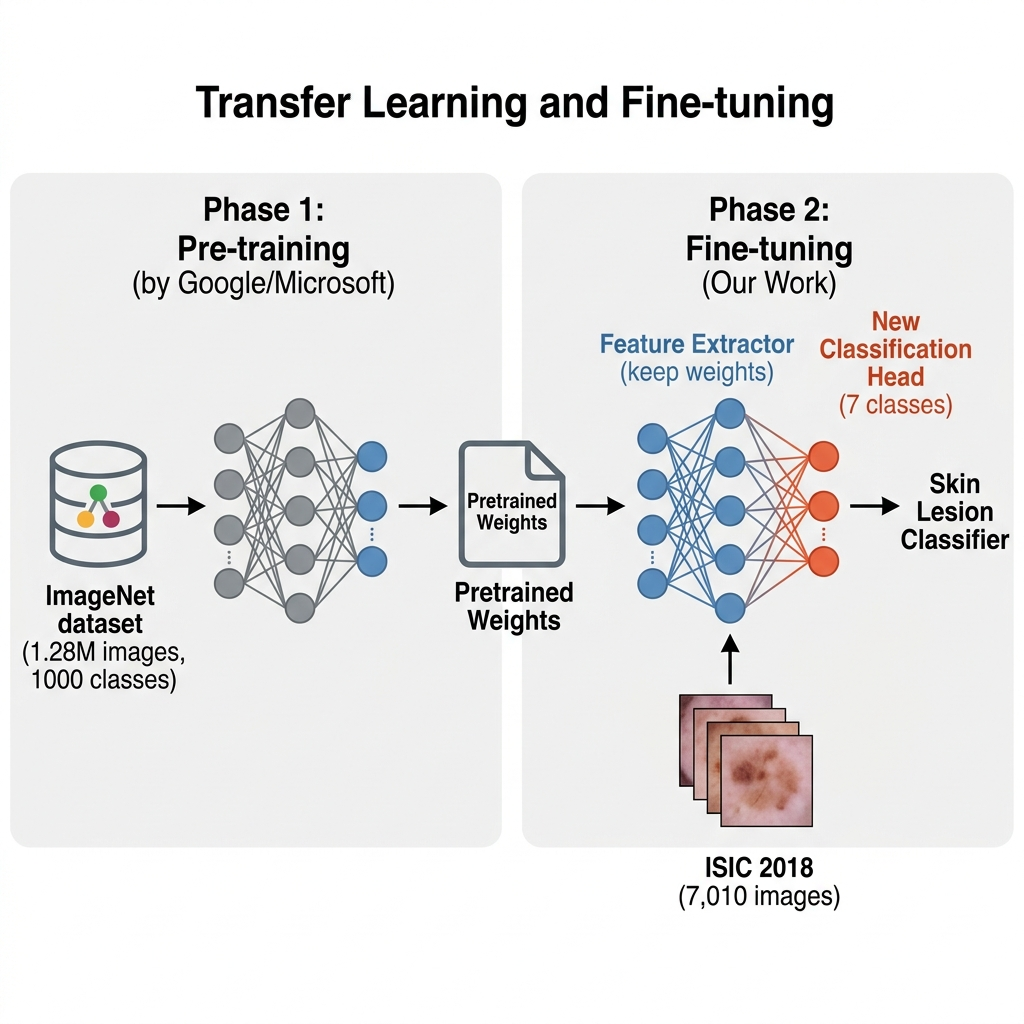
\includegraphics[width=0.85\textwidth]{thesis/figures/transfer_learning.png}\\
  \footnotesize \textit{Sơ đồ transfer learning: pretrain trên ImageNet $\rightarrow$ giữ feature extractor, thay classifier head, fine-tune trên ISIC 2018.}
\end{center}

% ===================================================
\section{Dữ liệu ISIC 2018}
% ===================================================

\subsection{Bộ dữ liệu HAM10000}

\textbf{ISIC 2018 Task 3} (tên khác: HAM10000) là benchmark chuẩn cho phân loại tổn thương da. Gồm \textbf{10.015 ảnh} dermoscopy chia thành 7 lớp:

\begin{table}[h]
\centering\small
\begin{tabular}{llrrrr}
\toprule
\textbf{Mã} & \textbf{Tên đầy đủ} & \textbf{Train} & \textbf{Val} & \textbf{Test} & \textbf{Tổng} \\
\midrule
nv     & Melanocytic Nevus (nốt ruồi)           & 4.693 & 1.006 & 1.006 & 6.705 \\
mel    & Melanoma (\textbf{ung thư hắc tố})     &   779 &   167 &   167 & 1.113 \\
bkl    & Benign Keratosis-like                  &   769 &   165 &   165 & 1.099 \\
bcc    & Basal Cell Carcinoma (ung thư biểu mô) &   360 &    77 &    77 &   514 \\
akiec  & Actinic Keratosis (tiền ung thư)       &   229 &    49 &    49 &   327 \\
vasc   & Vascular Lesion (tổn thương mạch máu)  &    99 &    21 &    22 &   142 \\
df     & Dermatofibroma (u xơ)                  &    81 &    17 &    17 &   115 \\
\midrule
\multicolumn{2}{l}{\textbf{Tổng}}                & 7.010 & 1.502 & 1.503 & \textbf{10.015} \\
\bottomrule
\end{tabular}
\end{table}

\subsection{Mất cân bằng dữ liệu --- vấn đề trung tâm}

Tỉ lệ lớp đông nhất (\texttt{nv}: 4.693) so với lớp ít nhất (\texttt{df}: 81) là \textbf{58:1}. Đây là \textit{vấn đề lâm sàng kinh điển} của mọi bài toán y tế: bệnh lý nguy hiểm như melanoma thường \textbf{hiếm} so với tổn thương lành tính.

\begin{idea}[Tại sao mất cân bằng là vấn đề lớn?]
Mạng nơ-ron tối thiểu hóa loss \textbf{trung bình}, nên ưu tiên lớp đông. Nếu không xử lý, mô hình có thể đạt 67\% Accuracy chỉ bằng cách dự đoán "nv" cho mọi ảnh --- nhưng \textbf{vô dụng lâm sàng} vì sẽ bỏ sót 100\% melanoma. Vì vậy ta dùng \textbf{Macro F1} làm metric chính: nó tính F1 trung bình \textit{không trọng số} của 7 lớp, ép mô hình quan tâm đến cả lớp hiếm.
\end{idea}

\subsection{Chia tập theo Stratified Sampling 70/15/15}

Tập gốc được chia tỉ lệ \textbf{70\% train / 15\% val / 15\% test} bằng \textit{stratified sampling}: mỗi split giữ nguyên tỉ lệ 7 lớp. Quan trọng để val/test có cùng phân phối với train --- nếu không, kết quả đo được sẽ không đáng tin.

\begin{center}
  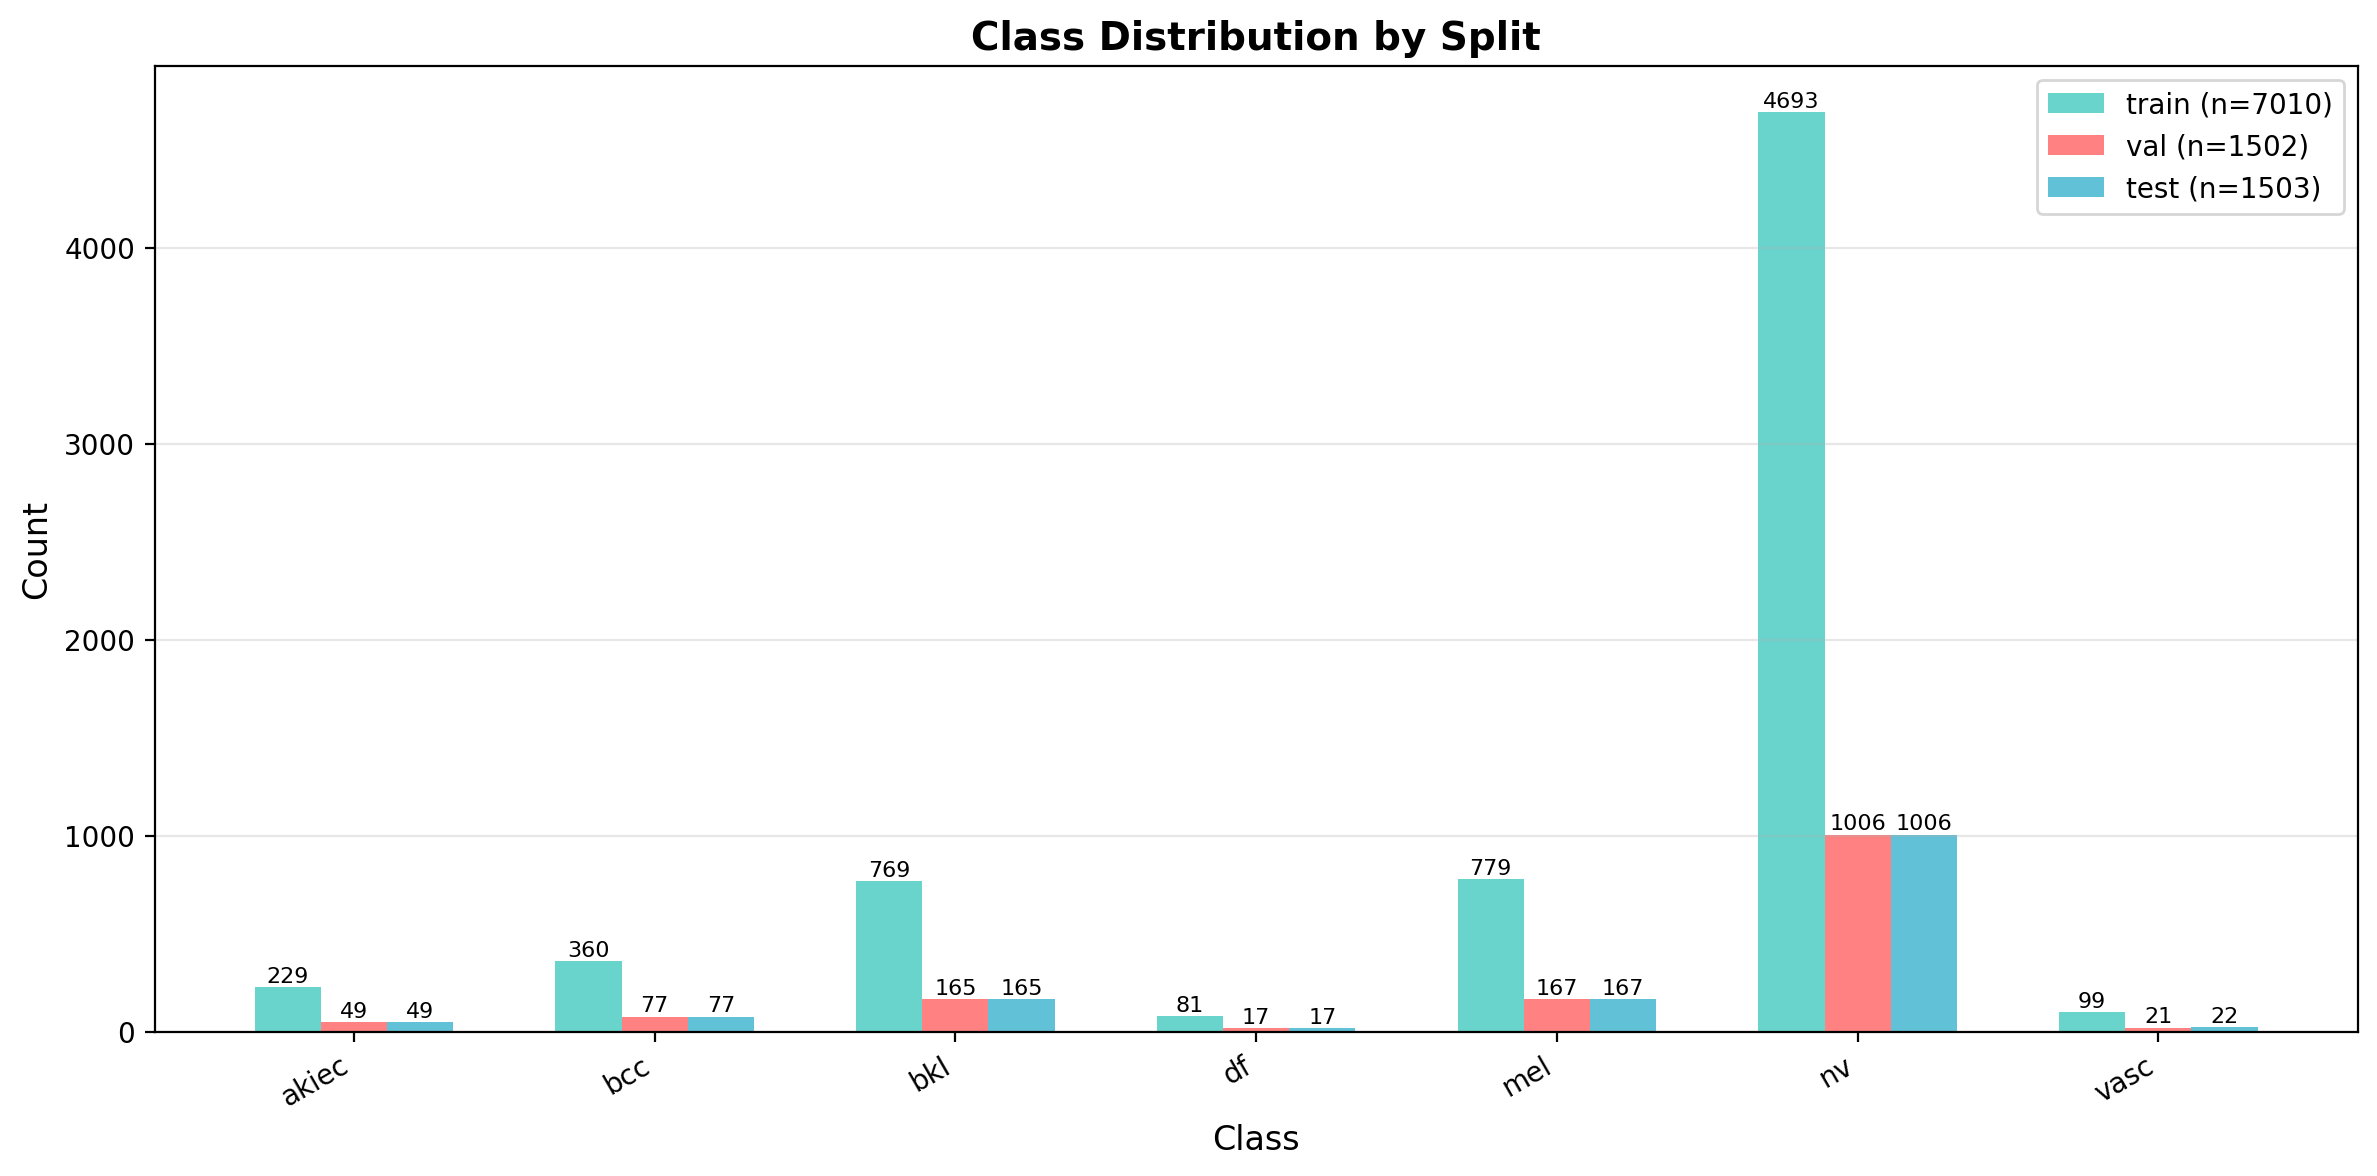
\includegraphics[width=0.8\textwidth]{thesis/figures/class_distribution.png}\\
  \footnotesize \textit{Phân bố 7 lớp giữ nguyên qua train/val/test (stratified split).}
\end{center}

% ===================================================
\section{Tiền xử lý và Augmentation}
% ===================================================

\subsection{Pipeline tổng quan}

\begin{center}
  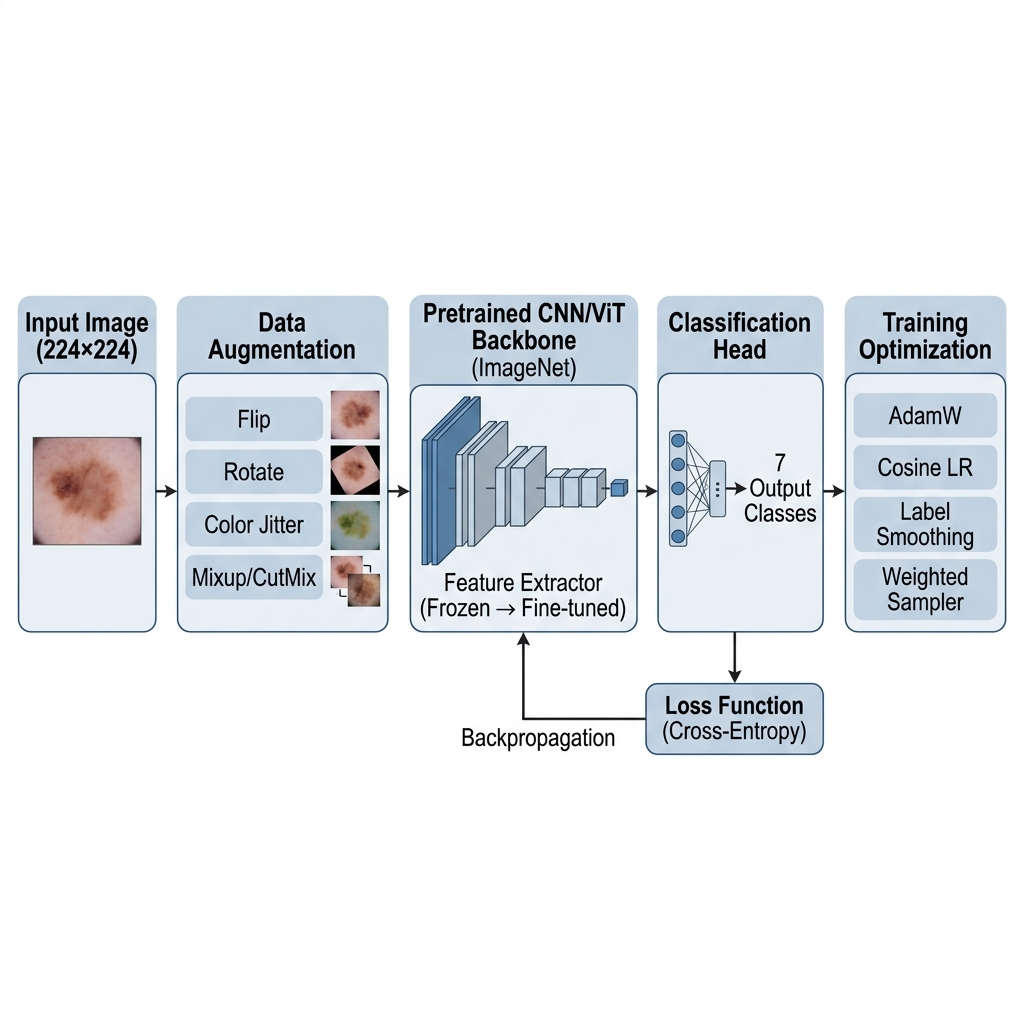
\includegraphics[width=0.95\textwidth]{thesis/figures/training_pipeline.png}\\
  \footnotesize \textit{Toàn bộ pipeline: ảnh thô $\to$ augmentation $\to$ backbone pretrained $\to$ classifier head $\to$ loss.}
\end{center}

\subsection{Tiền xử lý cơ bản}

Mọi ảnh đều được:
\begin{itemize}[leftmargin=*]
  \item \textbf{Resize} về $224 \times 224$ (kích thước input chuẩn cho ImageNet pretrained).
  \item \textbf{Chuyển sang tensor} (\texttt{ToTensor}) --- giá trị pixel $[0, 255] \to [0, 1]$.
  \item \textbf{Normalize} bằng mean/std của ImageNet:
  \[
    x' = \frac{x - \mu_{\text{ImageNet}}}{\sigma_{\text{ImageNet}}}, \quad
    \mu = (0.485, 0.456, 0.406), \quad
    \sigma = (0.229, 0.224, 0.225).
  \]
  \textit{Lý do dùng mean/std của ImageNet:} mô hình pretrained "kỳ vọng" input ở thang đo đó. Nếu normalize sai, distribution input lệch khỏi training distribution của ImageNet, hiệu năng tụt.
\end{itemize}

\subsection{Augmentation cho train set}

\textit{Augmentation} = biến đổi ngẫu nhiên ảnh train mỗi epoch để mô hình thấy nhiều "biến thể", giảm overfit. \textbf{Chỉ áp dụng trên train, không áp dụng trên val/test} (vì val/test cần phản ánh phân phối thực).

\begin{table}[h]
\centering\small
\begin{tabular}{lcc}
\toprule
\textbf{Phép biến đổi} & \textbf{Tham số} & \textbf{Lý do} \\
\midrule
RandomResizedCrop & scale 0.85--1.0   & Tăng scale invariance \\
HorizontalFlip    & $p=0.5$            & Ảnh da đối xứng theo trục \\
VerticalFlip      & $p=0.5$            & Ảnh dermoscopy không có "lên/xuống" cố định \\
Rotation          & $\pm 90^\circ$     & Bất biến theo xoay \\
ColorJitter       & b/c/s/h $= 0.25$   & Robust với khác biệt thiết bị \\
GaussianBlur      & $p=0.1$            & Robust với độ nét khác nhau \\
RandomErasing     & $p=0.1$            & Robust với che khuất \\
\bottomrule
\end{tabular}
\end{table}

\begin{lstlisting}[caption={\texttt{src/data/transforms.py} --- pipeline augmentation}]
def build_transforms(image_size, aug_cfg, is_train):
    normalize = transforms.Normalize(
        mean=[0.485, 0.456, 0.406],
        std =[0.229, 0.224, 0.225],
    )
    if is_train:
        train_tfms = [
            transforms.RandomResizedCrop(image_size, scale=(0.85, 1.0)),
            transforms.RandomHorizontalFlip(p=0.5),
            transforms.RandomVerticalFlip(p=0.5),
            transforms.RandomRotation(degrees=90),
            transforms.ColorJitter(brightness=0.25, contrast=0.25,
                                   saturation=0.25, hue=0.1),
            transforms.RandomApply([
                transforms.GaussianBlur(kernel_size=5, sigma=(0.1, 2.0)),
            ], p=0.1),
            transforms.ToTensor(),
            normalize,
            transforms.RandomErasing(p=0.1),
        ]
        return transforms.Compose(train_tfms)
    # Eval: chỉ resize + normalize
    return transforms.Compose([
        transforms.Resize((image_size, image_size)),
        transforms.ToTensor(), normalize,
    ])
\end{lstlisting}

% ===================================================
\section{Weighted Random Sampler}
% ===================================================

\subsection{Ý tưởng}

Thay vì để DataLoader chọn ảnh đều nhau, ta gán \textbf{trọng số} cho mỗi mẫu sao cho \textit{lớp hiếm được chọn thường xuyên hơn}. Mỗi mini-batch khi đó xấp xỉ cân bằng 7 lớp.

\subsection{Công thức}

Cho $N$ = tổng mẫu train, $C = 7$, $n_c$ = số mẫu lớp $c$. Trọng số mỗi mẫu thuộc lớp $c$:
\[
  w_c = \frac{1}{n_c} \quad \text{(hoặc dạng chuẩn hóa)} \quad w_c = \frac{N}{C \cdot n_c}.
\]

\begin{example}[Tính trọng số cụ thể trên ISIC 2018 train]
$N = 7.010$, $C = 7$. Bảng trọng số 7 lớp:
\begin{center}\small
\begin{tabular}{lrr}
\toprule
Lớp & $n_c$ & $w_c = N/(C\cdot n_c)$ \\
\midrule
nv   & 4.693 & 0.213 \\
mel  &   779 & 1.286 \\
bkl  &   769 & 1.303 \\
bcc  &   360 & 2.782 \\
akiec&   229 & 4.373 \\
vasc &    99 & \textbf{10.117} \\
df   &    81 & \textbf{12.365} \\
\bottomrule
\end{tabular}
\end{center}
\textbf{Hệ quả:} một ảnh \texttt{df} được DataLoader chọn với xác suất cao gấp $12.365 / 0.213 \approx \mathbf{58\times}$ so với một ảnh \texttt{nv}. Sau khi sampling, mini-batch xấp xỉ cân bằng.
\end{example}

\subsection{Code}

\begin{lstlisting}[caption={\texttt{src/data/samplers.py}}]
import numpy as np
import torch
from torch.utils.data import WeightedRandomSampler

def build_weighted_sampler(labels, num_classes):
    counts = np.bincount(labels, minlength=num_classes).astype(float)
    counts[counts == 0] = 1.0
    class_weights = 1.0 / counts                      # w_c
    sample_weights = [class_weights[lbl] for lbl in labels]
    sample_weights = torch.as_tensor(sample_weights, dtype=torch.double)
    return WeightedRandomSampler(
        weights=sample_weights,
        num_samples=len(sample_weights),
        replacement=True,
    )
\end{lstlisting}

% ===================================================
\section{Mixup}
% ===================================================

\subsection{Ý tưởng}

\textbf{Mixup} (Zhang et al., ICLR 2018) trộn \textit{tuyến tính} hai ảnh và hai nhãn của chúng để tạo một ảnh huấn luyện "ảo". Buộc mô hình hoạt động \textit{linearly} giữa các mẫu --- một dạng regularization rất mạnh.

\subsection{Công thức}

Cho hai mẫu $(x_i, y_i)$ và $(x_j, y_j)$. Lấy $\lambda \sim \mathrm{Beta}(\alpha, \alpha)$:
\[
  \tilde{x} = \lambda \, x_i + (1 - \lambda) \, x_j, \qquad
  \tilde{y} = \lambda \, y_i + (1 - \lambda) \, y_j.
\]

Trong đồ án $\alpha = 0.2$ $\Rightarrow$ $\lambda$ thường gần 0 hoặc 1, ít khi $\approx 0.5$. Nghĩa là Mixup pha trộn nhẹ, không phá ảnh quá mức.

\subsection{Ví dụ cụ thể}

\begin{example}[Mixup giữa 1 ảnh melanoma và 1 ảnh nevus]
\begin{itemize}[leftmargin=*]
  \item $x_i$ = ảnh melanoma, $y_i = $ \texttt{mel} (one-hot $[0,0,0,0,1,0,0]$)
  \item $x_j$ = ảnh nốt ruồi, $y_j = $ \texttt{nv} (one-hot $[0,0,0,0,0,1,0]$)
  \item Lấy $\lambda = 0.7$ ngẫu nhiên từ $\mathrm{Beta}(0.2, 0.2)$
\end{itemize}
\textbf{Ảnh trộn:} $\tilde{x} = 0.7 \, x_i + 0.3 \, x_j$ --- ảnh melanoma "rõ" 70\%, ảnh nốt ruồi "mờ" 30\% chồng lên.\\
\textbf{Nhãn trộn:} $\tilde{y} = 0.7 \cdot [0,0,0,0,1,0,0] + 0.3 \cdot [0,0,0,0,0,1,0] = [0,0,0,0,\mathbf{0.7},\mathbf{0.3},0]$\\
Mô hình phải dự đoán xác suất MEL gần $0.7$ và NV gần $0.3$.
\end{example}

\begin{note}
\textbf{Loss cho nhãn soft.} Cross-entropy thường dùng nhãn nguyên. Với nhãn lai, ta tính:
\[
  \mathcal{L} = \lambda \, \mathrm{CE}(f_\theta(\tilde{x}), y_i) + (1-\lambda) \, \mathrm{CE}(f_\theta(\tilde{x}), y_j).
\]
Tương đương loss với nhãn soft. Đây là logic của hàm \texttt{mixup\_criterion}.
\end{note}

\subsection{Code}

\begin{lstlisting}[caption={\texttt{src/data/mixup.py} --- hàm \texttt{mixup\_data}}]
def mixup_data(images, targets, alpha=0.2):
    lam = np.random.beta(alpha, alpha) if alpha > 0 else 1.0
    batch_size = images.size(0)
    index = torch.randperm(batch_size, device=images.device)

    mixed_images = lam * images + (1 - lam) * images[index]
    targets_a = targets
    targets_b = targets[index]
    return mixed_images, targets_a, targets_b, lam


def mixup_criterion(criterion, outputs, targets_a, targets_b, lam):
    """Loss cho nhãn lai."""
    return lam * criterion(outputs, targets_a) + \
           (1 - lam) * criterion(outputs, targets_b)
\end{lstlisting}

\subsection{Tại sao Mixup quan trọng?}

\begin{itemize}[leftmargin=*]
  \item Với chỉ 81 ảnh \texttt{df} trong train, không có Mixup mô hình sẽ \textit{ghi nhớ} các sample này trong vài epoch đầu.
  \item Mixup tạo ảnh mới mỗi batch, mô hình không thể "memorize" được.
  \item Làm mịn ranh giới quyết định, tránh over-confidence.
\end{itemize}

\textbf{Bằng chứng định lượng trong đồ án:} bỏ Mixup/CutMix khỏi pipeline làm Macro F1 \textit{giảm 4.51\%} --- đây là thành phần có đóng góp lớn nhất (xem \S\ref{sec:ablation}).

% ===================================================
\section{CutMix}
% ===================================================

\subsection{Ý tưởng}

\textbf{CutMix} (Yun et al., ICCV 2019) thay vì pha trộn toàn ảnh, ta \textbf{cắt một patch ngẫu nhiên} từ ảnh $j$ và \textit{dán lên} ảnh $i$. Nhãn lai theo \textit{tỉ lệ diện tích} patch dán so với ảnh.

\subsection{Công thức}

\[
  \tilde{x} = M \odot x_i + (1 - M) \odot x_j, \qquad
  \tilde{y} = \lambda \, y_i + (1-\lambda) \, y_j,
\]
trong đó:
\begin{itemize}[leftmargin=*]
  \item $M \in \{0,1\}^{H \times W}$ là mask bounding box ngẫu nhiên (1 = giữ pixel của $x_i$, 0 = lấy pixel của $x_j$).
  \item $\odot$ là tích element-wise.
  \item $\lambda = 1 - \dfrac{\text{diện tích patch}}{H \cdot W}$.
\end{itemize}

Trong đồ án $\alpha = 1.0$ $\Rightarrow$ $\lambda \sim \mathrm{Uniform}(0, 1)$, kích cỡ patch đa dạng.

\subsection{Ví dụ cụ thể}

\begin{example}[CutMix dán patch melanoma vào ảnh nevus]
\begin{itemize}[leftmargin=*]
  \item $x_i$ = ảnh nốt ruồi $224 \times 224$, $y_i = $ \texttt{nv}
  \item $x_j$ = ảnh melanoma $224 \times 224$, $y_j = $ \texttt{mel}
  \item Sample bounding box ngẫu nhiên size $80 \times 80$ ở góc trên-trái.
\end{itemize}
\textbf{Ảnh trộn:} ảnh nốt ruồi gốc, nhưng vùng $80 \times 80$ ở góc đã bị thay bằng pixel từ ảnh melanoma.\\
\textbf{Diện tích patch:} $80 \times 80 / (224 \times 224) = 0.128$\\
\textbf{$\lambda$:} $1 - 0.128 = 0.872$\\
\textbf{Nhãn trộn:} $0.872 \cdot y_{\text{nv}} + 0.128 \cdot y_{\text{mel}} = [0,0,0,0,\mathbf{0.128},\mathbf{0.872},0]$
\end{example}

\subsection{Code}

\begin{lstlisting}[caption={\texttt{src/data/mixup.py} --- hàm \texttt{cutmix\_data}}]
def cutmix_data(images, targets, alpha=1.0):
    lam = np.random.beta(alpha, alpha) if alpha > 0 else 1.0
    batch_size = images.size(0)
    index = torch.randperm(batch_size, device=images.device)

    _, _, H, W = images.shape
    cut_ratio = np.sqrt(1.0 - lam)
    cut_w = int(W * cut_ratio)
    cut_h = int(H * cut_ratio)

    cx = np.random.randint(W)
    cy = np.random.randint(H)
    x1 = max(0, cx - cut_w // 2); y1 = max(0, cy - cut_h // 2)
    x2 = min(W, cx + cut_w // 2); y2 = min(H, cy + cut_h // 2)

    mixed_images = images.clone()
    mixed_images[:, :, y1:y2, x1:x2] = images[index, :, y1:y2, x1:x2]

    # Cập nhật lambda theo diện tích thực sự
    lam = 1 - (y2 - y1) * (x2 - x1) / (H * W)

    return mixed_images, targets, targets[index], lam
\end{lstlisting}

\subsection{So sánh Mixup vs.\ CutMix}

\begin{table}[h]
\centering\small
\begin{tabular}{lll}
\toprule
& \textbf{Mixup} & \textbf{CutMix} \\
\midrule
Cách pha trộn  & Tuyến tính toàn ảnh   & Dán patch \\
Pixel gốc      & Bị phá vỡ              & Giữ nguyên trong patch \\
Tốt cho        & Smoothing biên quyết định & Features cục bộ \\
\bottomrule
\end{tabular}
\end{table}

Trong đồ án \textbf{áp dụng cả hai}, mỗi batch có xác suất 0.5 chọn 1 trong 2.

% ===================================================
\section{Label Smoothing}
% ===================================================

\subsection{Ý tưởng}

Mục tiêu của cross-entropy với nhãn one-hot là đẩy logit của lớp đúng về $+\infty$ và logit các lớp sai về $-\infty$ $\Rightarrow$ \textit{over-confidence}. \textbf{Label Smoothing} thay nhãn cứng bằng nhãn mềm, ép mô hình không "quá tự tin".

\subsection{Công thức}

\[
  y^{\text{LS}}_k = (1 - \varepsilon) \, \mathbb{1}[k = c] + \frac{\varepsilon}{C}, \qquad \varepsilon = 0.1, \; C = 7.
\]

\subsection{Ví dụ}

\begin{example}[Smoothing nhãn melanoma]
$y_{\text{onehot}} = [0, 0, 0, 0, 1, 0, 0]$ (lớp \texttt{mel} là 1, còn lại 0).

Với $\varepsilon = 0.1$, $C = 7$:
\begin{itemize}[leftmargin=*]
  \item Phần "đúng" giảm còn $1 - 0.1 = 0.9$
  \item Phần $0.1$ được \textit{rải đều} cho cả 7 lớp: mỗi lớp được $0.1 / 7 = 0.01429$
\end{itemize}
\[
  y^{\text{LS}} = [\mathbf{0.0143}, 0.0143, 0.0143, 0.0143, \mathbf{0.9143}, 0.0143, 0.0143].
\]
Đúng kiểm tra: tổng $= 0.9143 + 6 \times 0.0143 = 1.000$. ✓
\end{example}

\subsection{Tại sao hiệu quả}

\begin{itemize}[leftmargin=*]
  \item Không có Label Smoothing, model học đẩy logit lớp đúng $\to +\infty$ $\Rightarrow$ vector logit có magnitude lớn không cần thiết.
  \item Smoothing đặt cận trên cho logit đúng và cận dưới cho logit sai $\Rightarrow$ \textit{ranh giới quyết định mềm hơn}.
  \item Tốt cho các lớp tương đồng (MEL/NV/BKL) --- ranh giới cứng sẽ sai nhiều ở vùng biên.
\end{itemize}

\subsection{Code}

PyTorch tích hợp sẵn:

\begin{lstlisting}[caption={\texttt{src/models/losses.py}}]
import torch.nn as nn

def build_loss(loss_cfg, class_weights=None, device='cpu'):
    label_smoothing = float(loss_cfg.get('label_smoothing', 0.0))

    if loss_cfg['name'] == 'cross_entropy':
        return nn.CrossEntropyLoss(label_smoothing=label_smoothing)
    ...
\end{lstlisting}

\textbf{Một nghịch lý đã quan sát:} bỏ Label Smoothing làm AUC \textit{tăng} ($0.952 \to 0.967$) nhưng Macro F1 \textit{giảm} 3.11\%. Hard target $\Rightarrow$ model tự tin hơn (xếp hạng probability sắc nét $\Rightarrow$ AUC cao) nhưng ranh giới cứng làm sai ở vùng biên (F1 thấp).

% ===================================================
\section{Bốn kiến trúc mô hình được so sánh}
% ===================================================

\subsection{EfficientNet-B0 (5.3M tham số)}

\textbf{Ý tưởng chính:} \textit{compound scaling} --- đồng thời scale depth, width và resolution theo một hệ số chung. Sử dụng \textbf{MBConv} (Mobile Inverted Bottleneck) với \textit{depthwise separable convolution} và \textit{Squeeze-and-Excitation} (SE) để học global context theo kênh.

\textbf{Feature map cuối:} $(1280, 7, 7) \to$ GAP $\to$ \texttt{Linear(1280, 7)}.

\textbf{Vai trò trong đồ án:} mô hình \textbf{đơn lẻ tốt nhất} với chỉ 5.3M tham số (nhỏ nhất trong 4 mô hình).

\subsection{ResNet50 (25.6M tham số)}

\textbf{Ý tưởng chính:} \textit{residual connection} $f(x) = F(x) + x$ giúp mạng rất sâu vẫn huấn luyện được. Block \textit{bottleneck}: $1 \times 1$ giảm chiều $\to$ $3 \times 3$ conv $\to$ $1 \times 1$ tăng chiều.

\textbf{Feature map cuối:} $(2048, 7, 7) \to$ GAP $\to$ \texttt{Linear(2048, 7)}.

\subsection{DenseNet121 (8.0M tham số)}

\textbf{Ý tưởng chính:} \textit{dense connectivity} --- mỗi layer nhận concatenation của \textit{tất cả} layer trước đó. Tận dụng feature reuse, giảm số tham số.

\textbf{Feature map cuối:} $(1024, 7, 7) \to$ GAP $\to$ \texttt{Linear(1024, 7)}.

\subsection{Swin-Tiny (28.0M tham số)}

\textbf{Ý tưởng chính:} \textit{Shifted-window self-attention} --- chia ảnh thành các cửa sổ nhỏ, tính attention trong từng cửa sổ, rồi \textbf{dịch cửa sổ} để các vùng giao tiếp với nhau. Hierarchical 4 stage giống CNN: $56 \times 56 \to 28 \times 28 \to 14 \times 14 \to 7 \times 7$.

\textbf{Feature cuối:} $7 \times 7$ tokens $\times 768$ dim $\to$ global avg $\to$ \texttt{Linear(768, 7)}.

\textbf{Vai trò trong đồ án:} đại diện kiến trúc Transformer trong ensemble --- cung cấp \textit{ngữ cảnh toàn cục} (global self-attention), bù cho CNN vốn focus local.

\subsection{Tóm tắt}

\begin{table}[h]
\centering\small
\begin{tabular}{lcll}
\toprule
\textbf{Mô hình} & \textbf{Params} & \textbf{Nguyên tắc thiết kế} & \textbf{Vai trò ensemble} \\
\midrule
EfficientNet-B0 & 5.3M  & MBConv + SE, compound scaling     & CNN gọn, local features \\
ResNet50        & 25.6M & Bottleneck residual                & CNN sâu, baseline \\
DenseNet121     & 8.0M  & Dense connectivity, feature reuse  & CNN tận dụng feature reuse \\
Swin-Tiny       & 28.0M & Shifted-window self-attention      & Transformer, global context \\
\bottomrule
\end{tabular}
\end{table}

% ===================================================
\section{Huấn luyện}
% ===================================================

\subsection{Hàm mất mát}

Cross-entropy với label smoothing (\S 8):
\[
  \mathcal{L}_{\text{CE}}(p, y) = -\sum_{k=1}^C y^{\text{LS}}_k \log p_k.
\]

\subsection{Optimizer: AdamW}

\textbf{AdamW} (Loshchilov \& Hutter, 2019) = Adam với weight decay \textit{đúng cách} (decay áp dụng trực tiếp lên tham số, không vào gradient).

\[
  m_t = \beta_1 m_{t-1} + (1 - \beta_1) g_t, \quad
  v_t = \beta_2 v_{t-1} + (1 - \beta_2) g_t^2,
\]
\[
  \theta_t = \theta_{t-1} - \eta \left( \frac{\hat{m}_t}{\sqrt{\hat{v}_t} + \epsilon} + \lambda \theta_{t-1} \right).
\]

\subsection{Scheduler: Cosine Annealing với Warmup}

Giai đoạn đầu (\textbf{warmup}, 3--5 epoch): LR tăng tuyến tính từ 0 lên giá trị đỉnh, tránh phá vỡ pretrained weights.

Sau đó (\textbf{cosine}): LR giảm theo $\eta(t) = \eta_{\min} + \frac{1}{2}(\eta_{\max} - \eta_{\min})(1 + \cos(\pi t / T))$.

\subsection{Siêu tham số}

\begin{table}[h]
\centering\small
\begin{tabular}{lcccc}
\toprule
\textbf{Hyperparameter} & \textbf{EB0} & \textbf{RN50} & \textbf{DN121} & \textbf{Swin-Tiny} \\
\midrule
Learning rate       & 3e-4  & 3e-4 & 2.5e-4 & \textbf{1e-4} \\
Weight decay        & 1e-3  & 1e-3 & 1e-3   & \textbf{5e-2} \\
Warmup epochs       & 3     & 3    & 3      & 5 \\
Max epochs          & 50    & 50   & 50     & 50 \\
Batch size          & 16    & 16   & 16     & 16 \\
Mixup / CutMix $\alpha$ & 0.2 / 1.0 & 0.2 / 1.0 & 0.2 / 1.0 & 0.2 / 1.0 \\
Label smoothing $\varepsilon$ & 0.1 & 0.1 & 0.1 & 0.1 \\
\bottomrule
\end{tabular}
\end{table}

\textbf{Tại sao Swin khác?} Transformer thiếu \textit{inductive bias} của CNN $\Rightarrow$ cần LR thấp để không phá pretrained attention weights, và weight decay cao để hạn chế overfit (28M tham số trên 7K ảnh = tỉ lệ rất dễ overfit).

\subsection{Vòng lặp huấn luyện}

\begin{lstlisting}[caption={\texttt{src/engine/train\_eval.py} (rút gọn)}]
def train_one_epoch(model, loader, optimizer, criterion, scaler, ...):
    model.train()
    for batch in loader:
        images, targets, _ = batch
        images, targets = images.to(device), targets.to(device)

        # Mixup hoặc CutMix với xác suất 0.5
        r = np.random.rand()
        if r < 0.5:
            images, targets_a, targets_b, lam = mixup_data(
                images, targets, alpha=0.2)
        else:
            images, targets_a, targets_b, lam = cutmix_data(
                images, targets, alpha=1.0)

        with torch.cuda.amp.autocast():  # Mixed precision FP16
            outputs = model(images)
            loss = mixup_criterion(
                criterion, outputs, targets_a, targets_b, lam)

        scaler.scale(loss).backward()
        scaler.unscale_(optimizer)
        torch.nn.utils.clip_grad_norm_(model.parameters(), 1.0)  # grad clip
        scaler.step(optimizer)
        scaler.update()
        optimizer.zero_grad()
\end{lstlisting}

\textbf{Mixed precision (FP16):} tính toán bằng float 16-bit thay 32-bit $\Rightarrow$ giảm $\sim$40\% bộ nhớ GPU, tăng tốc $\sim$1.5--2$\times$, mà không mất accuracy.

% ===================================================
\section{Ensemble bằng Soft Voting}
% ===================================================

\subsection{Tại sao cần ensemble?}

Mỗi mô hình \textit{sai ở những chỗ khác nhau}. CNN focus local features, Swin focus global context $\Rightarrow$ lỗi không tương quan. Trung bình các dự đoán \textit{giảm phương sai dự đoán} mà không tăng bias.

\subsection{Soft voting --- công thức}

Với $M = 4$ mô hình, mỗi mô hình $m$ cho vector xác suất $p_m(x) \in [0, 1]^C$:
\[
  \bar{p}(x) = \frac{1}{M} \sum_{m=1}^{M} p_m(x), \qquad
  \hat{y} = \arg\max_c \bar{p}_c(x).
\]

\subsection{Ví dụ cụ thể}

\begin{example}[Soft voting trên 1 ảnh test]
Cho 1 ảnh dermoscopy thật, 4 mô hình cho 4 vector xác suất sau (cho 7 lớp \texttt{akiec, bcc, bkl, df, mel, nv, vasc}):

\small
\begin{tabular}{lccccccc}
\toprule
& akiec & bcc & bkl & df & \textbf{mel} & nv & vasc \\
\midrule
EB0    & 0.02 & 0.03 & 0.05 & 0.01 & \textbf{0.65} & 0.22 & 0.02 \\
RN50   & 0.03 & 0.05 & 0.08 & 0.01 & \textbf{0.55} & 0.26 & 0.02 \\
DN121  & 0.02 & 0.03 & 0.06 & 0.01 & \textbf{0.62} & 0.24 & 0.02 \\
Swin   & 0.04 & 0.04 & 0.05 & 0.01 & \textbf{0.48} & 0.36 & 0.02 \\
\midrule
\textbf{TB} & 0.028 & 0.038 & 0.060 & 0.010 & \textbf{0.575} & 0.270 & 0.020 \\
\bottomrule
\end{tabular}
\normalsize

\textbf{Argmax:} \texttt{mel} với xác suất ensemble 57.5\%. Cả 4 mô hình \textit{đều} chỉ ra MEL, Swin "chưa chắc lắm" (48\%) nhưng các CNN khác đẩy lên --- kết quả ensemble vẫn vững.
\end{example}

\subsection{Tại sao soft voting hiệu quả? --- Phân rã bias--variance}

\[
  \mathbb{E}\bigl[(\bar{p} - y)^2\bigr] = \underbrace{\overline{\mathrm{bias}^2}}_{\text{cố định}} + \underbrace{\frac{1}{M}\overline{\mathrm{var}}}_{\text{giảm }M\text{ lần nếu độc lập}} + \underbrace{\frac{M-1}{M}\overline{\mathrm{cov}}}_{\text{covariance dư}}
\]

\begin{itemize}[leftmargin=*]
  \item Bias giữ nguyên (vì các mô hình học cùng task).
  \item Variance giảm theo $1/M$ \textit{nếu} lỗi độc lập.
  \item \textbf{Chìa khóa:} CNN (local) và Swin (global) có covariance lỗi thấp $\Rightarrow$ ensemble thật sự cải thiện.
\end{itemize}

\subsection{Code}

\begin{lstlisting}[caption={\texttt{src/ensemble.py} --- core logic}]
import numpy as np
import torch
import torch.nn.functional as F

# Mỗi mô hình → 1 ma trận xác suất (N × 7)
probs_eb0   = run_inference(model_eb0,   test_loader)   # (1503, 7)
probs_rn50  = run_inference(model_rn50,  test_loader)
probs_dn121 = run_inference(model_dn121, test_loader)
probs_swin  = run_inference(model_swin,  test_loader)

# Stack và trung bình
stacked = np.stack([probs_eb0, probs_rn50, probs_dn121, probs_swin])
# shape: (4, 1503, 7)
avg_probs = stacked.mean(axis=0)            # (1503, 7)

# Dự đoán cuối
y_pred = avg_probs.argmax(axis=1)           # (1503,)
\end{lstlisting}

\subsection{So sánh với phương án khác}

\begin{table}[h]
\centering\small
\begin{tabular}{lll}
\toprule
\textbf{Phương án} & \textbf{Cách làm} & \textbf{Hạn chế} \\
\midrule
Soft voting (chọn)   & Trung bình xác suất     & --- \\
Hard voting          & Mỗi model argmax rồi vote & Mất thông tin xác suất \\
Stacking             & Meta-learner học trọng số & Cần val riêng, overfit \\
\bottomrule
\end{tabular}
\end{table}

\begin{center}
  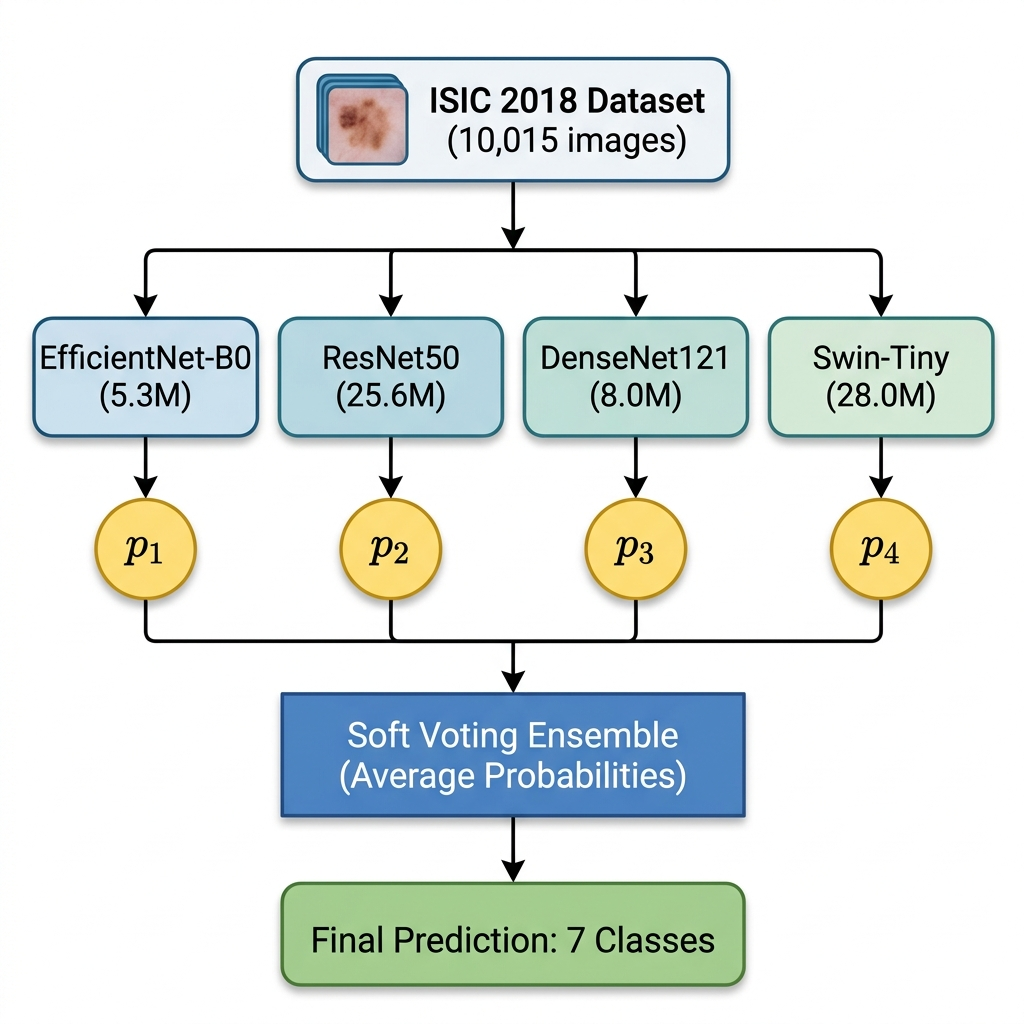
\includegraphics[width=0.65\textwidth]{thesis/figures/ensemble_architecture.png}
\end{center}

% ===================================================
\section{Grad-CAM --- khả diễn giải}
% ===================================================

\subsection{Tại sao Grad-CAM xài được?}

Khi mạng CNN/Transformer dự đoán lớp $c$ với xác suất $p_c$, ta muốn biết \textit{vùng nào trên ảnh đã đóng góp vào quyết định đó}. Ý tưởng cốt lõi:
\begin{itemize}[leftmargin=*]
  \item Activation map $A^k$ ở layer conv cuối cùng chứa thông tin spatial (vẫn còn dạng $H \times W$).
  \item Gradient $\partial y_c / \partial A^k$ cho biết \textit{kênh $k$ tăng thì xác suất lớp $c$ tăng bao nhiêu}.
  \item Trung bình gradient toàn không gian (\textit{global average pooling}) cho ra trọng số $\alpha_c^k$.
  \item Trọng số $\alpha_c^k$ kết hợp với activation $A^k$ $\Rightarrow$ heatmap.
\end{itemize}

\subsection{Bốn bước toán học}

Cho ảnh đầu vào $x$, lớp mục tiêu $c$, feature map $A \in \mathbb{R}^{K \times H \times W}$ tại layer cuối:

\textbf{Bước 1 --- forward $+$ backward:}
\[
  y^c = f_\theta(x)[c], \qquad \frac{\partial y^c}{\partial A^k_{ij}} \quad (\text{lấy bằng PyTorch hooks}).
\]

\textbf{Bước 2 --- trọng số kênh (global average pooling gradient):}
\[
  \alpha_c^k = \frac{1}{HW} \sum_{i=1}^H \sum_{j=1}^W \frac{\partial y^c}{\partial A^k_{ij}}.
\]

\textbf{Bước 3 --- heatmap (chỉ giữ phần positive):}
\[
  L_c = \mathrm{ReLU}\left( \sum_{k=1}^K \alpha_c^k \, A^k \right) \in \mathbb{R}^{H \times W}.
\]

\textbf{Bước 4 --- upsample + overlay:} Up-sample $L_c$ về $224 \times 224$ bằng nội suy bilinear, chuẩn hóa $[0, 1]$, áp colormap JET (đỏ = cao, xanh = thấp), overlay lên ảnh gốc.

\subsection{Trực giác}

\begin{itemize}[leftmargin=*]
  \item $\alpha_c^k$ \textit{lớn dương} $\Rightarrow$ kênh $k$ đóng góp positive cho lớp $c$.
  \item Kết hợp $\sum \alpha_c^k A^k$ cho biết \textit{vị trí trong feature map} mà các kênh quan trọng đang "phát sáng".
  \item ReLU loại bỏ phần đóng góp âm (vùng làm \textit{giảm} xác suất $c$) --- chỉ giữ bằng chứng tích cực.
\end{itemize}

\subsection{Code GradCAM class}

\begin{lstlisting}[caption={\texttt{src/utils/grad\_cam.py} --- rút gọn}]
class GradCAM:
    def __init__(self, model, target_layer):
        self.model = model
        self.target_layer = target_layer
        self.activations = None
        self.gradients   = None
        # Hooks ghi lại activation forward và gradient backward
        target_layer.register_forward_hook(self._save_activation)
        target_layer.register_full_backward_hook(self._save_gradient)

    def _save_activation(self, _module, _input, output):
        self.activations = output.detach()

    def _save_gradient(self, _module, _grad_input, grad_output):
        self.gradients = grad_output[0].detach()

    @torch.enable_grad()
    def __call__(self, input_tensor, target_class=None):
        input_tensor = input_tensor.requires_grad_(True)
        # 1. Forward
        output = self.model(input_tensor)
        probs  = F.softmax(output, dim=1)
        if target_class is None:
            target_class = output.argmax(dim=1).item()

        # 2. Backward
        self.model.zero_grad()
        output[0, target_class].backward()

        # 3. Trọng số kênh = GAP gradient
        gradients   = self.gradients[0]    # (C, H, W)
        activations = self.activations[0]  # (C, H, W)
        weights     = gradients.mean(dim=(1, 2))   # (C,)

        # 4. Weighted sum + ReLU
        cam = torch.zeros(activations.shape[1:], device=activations.device)
        for k, w in enumerate(weights):
            cam += w * activations[k]
        cam = F.relu(cam)

        # 5. Normalize [0, 1]
        cam = cam - cam.min()
        if cam.max() > 0:
            cam = cam / cam.max()
        return cam.cpu().numpy(), target_class, probs[0, target_class].item()
\end{lstlisting}

\subsection{Target layer mỗi mô hình khác nhau --- tại sao?}

\begin{table}[h]
\centering\small
\begin{tabular}{llcl}
\toprule
\textbf{Mô hình} & \textbf{Target layer} & \textbf{Kích thước} & \textbf{Lý do} \\
\midrule
EfficientNet-B0 & \texttt{model.blocks[-1][-1]}    & (320, 7, 7) & MBConv cuối, depthwise 3$\times$3 \\
ResNet50        & \texttt{model.layer4[-1]}        & (2048, 7, 7) & Residual block cuối \\
DenseNet121     & \texttt{model.features.norm5}    & (1024, 7, 7) & BatchNorm sau dense block cuối \\
Swin-Tiny       & \texttt{model.layers[-1].blocks[-1].norm2} & (49, 768) & LayerNorm sau attention cuối \\
\bottomrule
\end{tabular}
\end{table}

\begin{idea}[Bài học từ EfficientNet --- không dùng \texttt{model.bn2}]
Ban đầu code dùng \texttt{model.bn2} (BatchNormAct2d $+$ SiLU). SiLU$(x) \approx 0$ với $x < 0$, sau BN khoảng 50\% activation về 0 $\Rightarrow$ chỉ 18\% pixel có activation $\Rightarrow$ heatmap xanh đồng đều, không tập trung.

Chuyển sang \texttt{model.blocks[-1][-1]}: 51\% pixel active, kết quả khoanh đúng tổn thương.
\end{idea}

\subsection{Grad-CAM định lượng}

Chỉ nhìn heatmap thì cảm tính. Để \textit{chứng minh} mô hình focus đúng tổn thương, ta đo các chỉ số sau (so với mask lesion sinh từ Otsu threshold):

\begin{table}[h]
\centering\small
\begin{tabular}{lp{9cm}}
\toprule
\texttt{focus\_ratio}       & Tỉ lệ tổng activation nằm trong mask lesion. Cao $\Rightarrow$ focus đúng chỗ. \\
\texttt{mean\_act\_in/out}  & Cường độ trung bình trong/ngoài mask. \\
\texttt{entropy}            & Shannon entropy của heatmap. Thấp $\Rightarrow$ focus sắc nét. \\
\texttt{peak\_distance}     & Khoảng cách từ peak activation tới centroid lesion (normalize). \\
\texttt{coverage\_75}       & \% diện tích chứa 25\% activation cao nhất. Thấp $\Rightarrow$ compact. \\
\bottomrule
\end{tabular}
\end{table}

Cả 4 mô hình đạt \texttt{focus\_ratio} > 0.6 và \texttt{peak\_distance} < 0.2 trên test set.

\begin{center}
  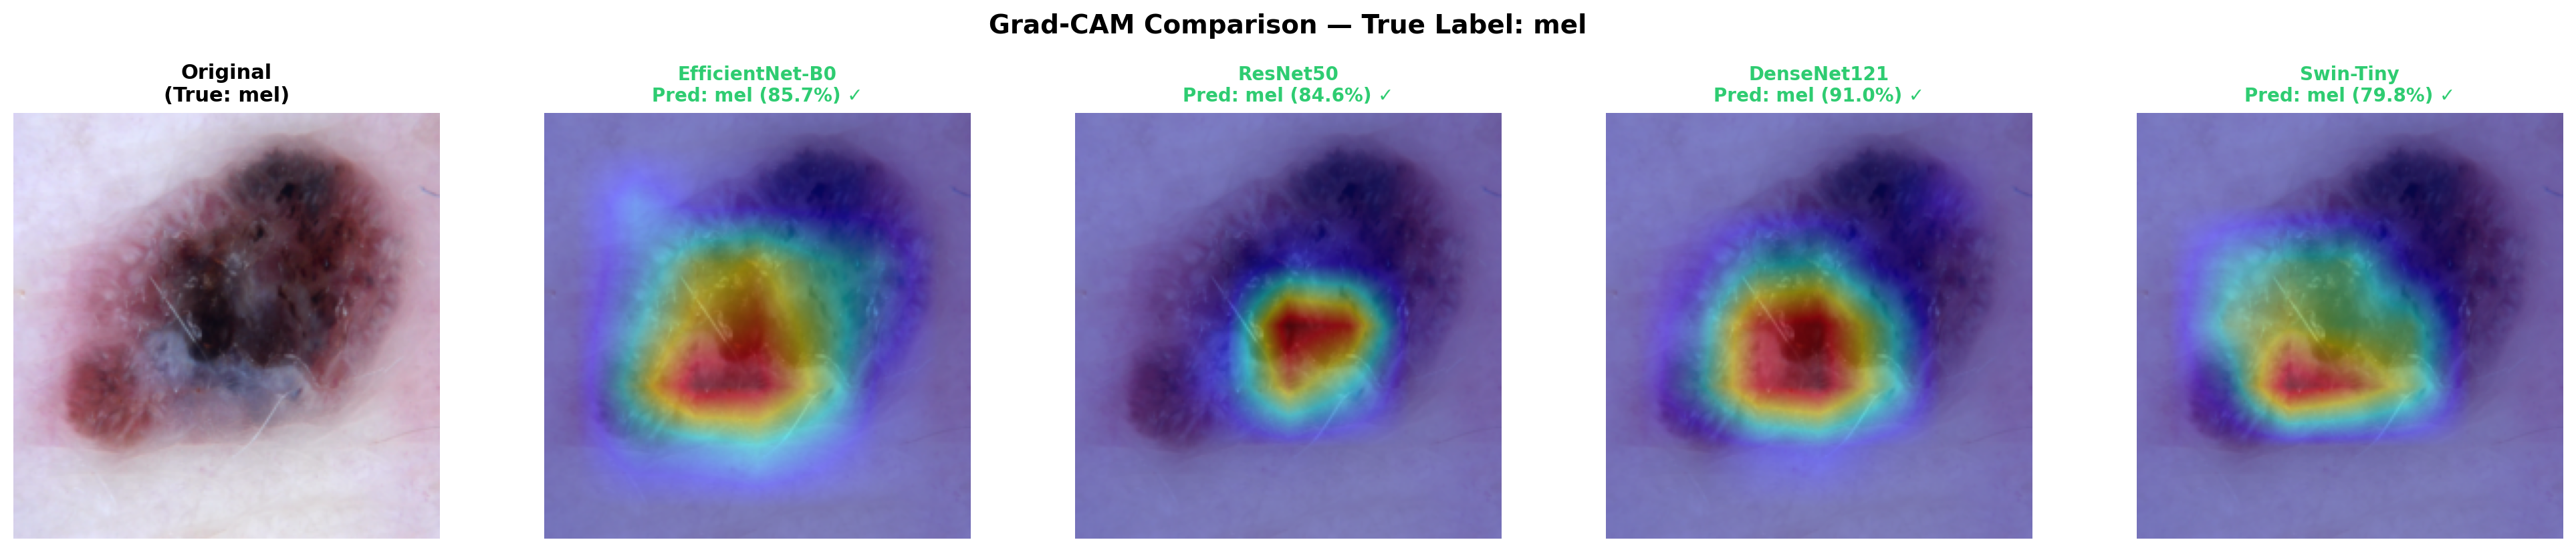
\includegraphics[width=0.85\textwidth]{thesis/figures/gradcam_mel_sample.png}\\
  \footnotesize \textit{Grad-CAM trên một mẫu melanoma --- cả 4 mô hình đều khoanh đúng ổ sắc tố trung tâm.}
\end{center}

% ===================================================
\section{Các chỉ số đánh giá}
% ===================================================

\subsection{Tại sao Accuracy không đủ?}

Trên ISIC 2018, một mô hình "đoán \texttt{nv} cho mọi ảnh" đạt $\sim$67\% Accuracy nhưng \textit{bỏ sót 100\% melanoma}. Vì vậy ta dùng các metric \textbf{bình đẳng với mọi lớp}.

\subsection{Định nghĩa từng chỉ số}

\begin{table}[h]
\centering\small
\begin{tabular}{lll}
\toprule
\textbf{Chỉ số} & \textbf{Công thức} & \textbf{Ý nghĩa} \\
\midrule
Accuracy        & $\sum_c TP_c / N$                                  & Tỉ lệ đúng tổng thể (lệch trên data imbalance) \\
Macro F1        & $\frac{1}{C}\sum_c F1_c$                           & F1 trung bình không trọng số \\
Weighted F1     & $\sum_c F1_c \cdot n_c / N$                        & F1 có trọng số theo cỡ lớp \\
Macro AUC       & $\frac{1}{C}\sum_c \mathrm{AUC}_c$ (One-vs-Rest)   & Khả năng xếp hạng xác suất \\
Cohen's $\kappa$ & $(P_o - P_e)/(1 - P_e)$                           & Đồng thuận so với random \\
MCC             & $\frac{TP \cdot TN - FP \cdot FN}{\sqrt{(\dots)}}$ & Cân bằng nhất, dùng cả 4 ô confusion \\
Sensitivity     & $TP/(TP+FN)$                                       & Recall --- phát hiện đúng positive \\
Specificity     & $TN/(TN+FP)$                                       & Xác định đúng negative \\
\bottomrule
\end{tabular}
\end{table}

\subsection{Ví dụ tính F1, Precision, Recall}

\begin{example}[Tính F1 cho lớp MEL trên ensemble]
Trên test set có \textbf{167 ảnh MEL thật}. Ensemble dự đoán "MEL" cho \textbf{166 ảnh}, trong đó \textbf{124 ảnh đúng là MEL}.
\begin{align*}
  TP &= 124, \quad FP = 166 - 124 = 42, \quad FN = 167 - 124 = 43 \\[2pt]
  \mathrm{Precision} &= \frac{TP}{TP + FP} = \frac{124}{166} = 0.747 \\[2pt]
  \mathrm{Recall (Sensitivity)} &= \frac{TP}{TP + FN} = \frac{124}{167} = 0.740 \\[2pt]
  F1 &= \frac{2 \cdot P \cdot R}{P + R} = \frac{2 \cdot 0.747 \cdot 0.740}{0.747 + 0.740} = \mathbf{0.744}
\end{align*}
\end{example}

\subsection{Tại sao Sensitivity cho MEL được ưu tiên?}

Trong y tế, \textbf{bỏ sót} một melanoma (false negative) nguy hiểm hơn \textbf{báo động giả} (false positive). False positive làm bệnh nhân thêm xét nghiệm; false negative làm bệnh nhân chết. Vì vậy khi triển khai, ta có thể \textit{hạ ngưỡng quyết định MEL} để tăng sensitivity.

% ===================================================
\section{Ablation Study}\label{sec:ablation}
% ===================================================

\subsection{Phương pháp}

\textit{Ablation} = lần lượt \textbf{bỏ một thành phần} của pipeline để đo mức suy giảm hiệu năng $\Rightarrow$ xác định thành phần nào quan trọng nhất. Baseline = EfficientNet-B0 với pipeline đầy đủ.

\subsection{Kết quả}

\begin{table}[h]
\centering\small
\begin{tabular}{lcccc}
\toprule
\textbf{Cấu hình} & \textbf{Accuracy} & \textbf{Macro F1} & \textbf{AUC} & \textbf{$\Delta$ F1} \\
\midrule
\textbf{Full pipeline (baseline)} & \textbf{0.8836} & \textbf{0.8311} & 0.9522 & --- \\
\midrule
$-$ Mixup \& CutMix          & 0.8589 & 0.7860 & 0.9486 & \textcolor{red}{$\mathbf{-0.0451}$} \\
$-$ Label Smoothing          & 0.8776 & 0.8000 & \textbf{0.9674} & \textcolor{red}{$-0.0311$} \\
$-$ Weighted Sampler         & 0.8762 & 0.8041 & 0.9521 & \textcolor{red}{$-0.0270$} \\
$-$ Advanced Augmentation    & \textbf{0.8896} & 0.8204 & 0.9664 & \textcolor{red}{$-0.0107$} \\
\bottomrule
\end{tabular}
\end{table}

\subsection{Diễn giải từng thành phần}

\textbf{1. Mixup/CutMix (quan trọng nhất, $-4.51$\% F1).} Với chỉ 81 ảnh DF và 99 ảnh VASC, không có Mixup/CutMix mô hình memorize sample hiếm.

\textbf{2. Nghịch lý Label Smoothing.} Bỏ Label Smoothing \textit{tăng} AUC ($0.952 \to 0.967$) nhưng \textit{giảm} F1 (3.11\%). Hard target $\Rightarrow$ probability ranking sắc nét hơn (AUC cao) nhưng ranh giới cứng sai nhiều ở MEL/NV/BKL (F1 thấp).

\textbf{3. Weighted Sampler ($-2.70$\% F1).} Không sampler, model học chủ yếu từ NV, recall của DF/VASC/AKIEC sụt rõ rệt.

\textbf{4. Trade-off Augmentation.} Bỏ aug mạnh, Accuracy thậm chí \textit{nhỉnh hơn} (88.96\% > 88.36\%) vì model dễ fit NV hơn. Nhưng Macro F1 giảm --- minority class bị bỏ rơi.

\begin{idea}[Bài học chính từ ablation]
Đóng góp lớn nhất \textbf{không phải kiến trúc lớn hơn} mà \textbf{regularization tốt hơn}. Mixup/CutMix $+$ Label Smoothing đóng góp tổng cộng 7.62\% F1 --- nhiều hơn khoảng cách giữa các kiến trúc.
\end{idea}

% ===================================================
\section{Kết quả thực nghiệm chính}
% ===================================================

\subsection{Bảng so sánh 4 mô hình đơn + Ensemble}

\begin{table}[h]
\centering\small
\begin{tabular}{lcccccc}
\toprule
\textbf{Mô hình} & \textbf{Params} & \textbf{Epoch tốt} & \textbf{Acc} & \textbf{Macro F1} & \textbf{AUC} & \textbf{Kappa} \\
\midrule
\textbf{EfficientNet-B0} & \textbf{5.3M} & 39 & \textbf{0.8836} & \textbf{0.8311} & 0.9522 & \textbf{0.7710} \\
ResNet50                 & 25.6M & 39 & 0.8603 & 0.7902 & 0.9565 & 0.7309 \\
DenseNet121              & 8.0M  & 49 & 0.8543 & 0.7967 & 0.9587 & 0.7206 \\
Swin-Tiny                & 28.0M & \textbf{13} & 0.8490 & 0.7855 & \textbf{0.9600} & 0.7150 \\
\midrule
\rowcolor{usthblue!10}
\textbf{Ensemble} & --- & --- & \textbf{0.8949} & \textbf{0.8446} & \textbf{0.9802} & --- \\
\bottomrule
\end{tabular}
\end{table}

\subsection{Độ tin cậy thống kê (multi-seed)}

Số liệu trên ở 1 hạt giống đại diện (42). Để chứng minh không phải may mắn, ta lặp lại toàn bộ pipeline với 5 hạt giống (\{42, 1337, 2024, 7, 11\}).

\begin{table}[h]
\centering\small
\begin{tabular}{lccc}
\toprule
\textbf{Mô hình} & \textbf{Accuracy} & \textbf{Macro F1} & \textbf{Macro AUC} \\
\midrule
EfficientNet-B0 & $87{,}31 \pm 1{,}32\%$ & $0{,}814 \pm 0{,}022$ & $0{,}965 \pm 0{,}006$ \\
ResNet50        & $86{,}31 \pm 0{,}57\%$ & $0{,}792 \pm 0{,}011$ & $0{,}949 \pm 0{,}003$ \\
DenseNet121     & $85{,}62 \pm 2{,}42\%$ & $0{,}797 \pm 0{,}025$ & $0{,}960 \pm 0{,}004$ \\
Swin-Tiny       & $\mathbf{88{,}33 \pm 1{,}96\%}$ & $0{,}839 \pm 0{,}030$ & $0{,}966 \pm 0{,}008$ \\
\midrule
\rowcolor{usthblue!10}
\textbf{Ensemble} & $\mathbf{89{,}93 \pm 0{,}66\%}$ & $\mathbf{0{,}852 \pm 0{,}010}$ & $\mathbf{0{,}982 \pm 0{,}001}$ \\
\bottomrule
\end{tabular}
\end{table}

\begin{idea}[3 phát hiện quan trọng]
\textbf{(1)} Số gốc 89,49\% nằm trong 1$\sigma$ của trung bình 89,93\% --- xác nhận robust, không lucky.\\
\textbf{(2)} Swin-Tiny mới là mô hình đơn mạnh nhất khi average qua seeds (88,33\% > EB0 87,31\%). Hạt giống 42 là pha xui của Swin (early-stop sớm).\\
\textbf{(3)} Std của ensemble cực nhỏ (Acc 0,66\%, AUC 0,001) --- soft voting hấp thụ phương sai cấp hạt giống.
\end{idea}

\textbf{McNemar test (ensemble vs.\ mỗi mô hình đơn, Fisher tổ hợp 5 hạt giống):}

\begin{table}[h]
\centering\small
\begin{tabular}{lccc}
\toprule
\textbf{Mô hình đơn vs.\ Ensemble} & \textbf{Ensemble thắng} & \textbf{p Fisher tổ hợp} \\
\midrule
EfficientNet-B0 & 5/5 & $5{,}3 \times 10^{-18}$ \\
ResNet50        & 5/5 & $4{,}5 \times 10^{-31}$ \\
DenseNet121     & 5/5 & $6{,}7 \times 10^{-39}$ \\
Swin-Tiny (mạnh nhất) & 5/5 & $1{,}2 \times 10^{-7}$ \\
\bottomrule
\end{tabular}
\end{table}

Ensemble thắng \textbf{5/5 hạt giống} so với mọi backbone, p-value cực thấp --- bằng chứng thống kê mạnh cho hội đồng.

\subsection{Hiệu năng per-class của Ensemble}

\begin{table}[h]
\centering\small
\begin{tabular}{lrrrrrr}
\toprule
\textbf{Lớp} & \textbf{Support} & \textbf{Precision} & \textbf{Recall} & \textbf{F1} & \textbf{AUC} & \textbf{Specificity} \\
\midrule
AKIEC &   49 & 0.692 & 0.735 & 0.710 & 0.972 & 0.989 \\
BCC   &   77 & 0.875 & 0.779 & 0.825 & 0.996 & 0.994 \\
BKL   &  165 & 0.792 & 0.800 & 0.796 & 0.968 & 0.974 \\
DF    &   17 & 0.938 & 0.938 & 0.938 & 0.996 & 0.999 \\
\textbf{MEL} &  167 & \textbf{0.747} & \textbf{0.740} & \textbf{0.744} & \textbf{0.958} & \textbf{0.968} \\
NV    & 1.006 & 0.950 & 0.942 & 0.946 & 0.972 & 0.901 \\
VASC  &   22 & 1.000 & 0.913 & 0.955 & 1.000 & 1.000 \\
\midrule
\textbf{Macro avg} & --- & 0.856 & 0.835 & 0.845 & 0.980 & 0.975 \\
\bottomrule
\end{tabular}
\end{table}

Tất cả 7 lớp đều có F1 > 0.70 --- \textit{không có lớp nào bị bỏ rơi}, kể cả DF và VASC chỉ 17 và 22 mẫu test.

\begin{center}
  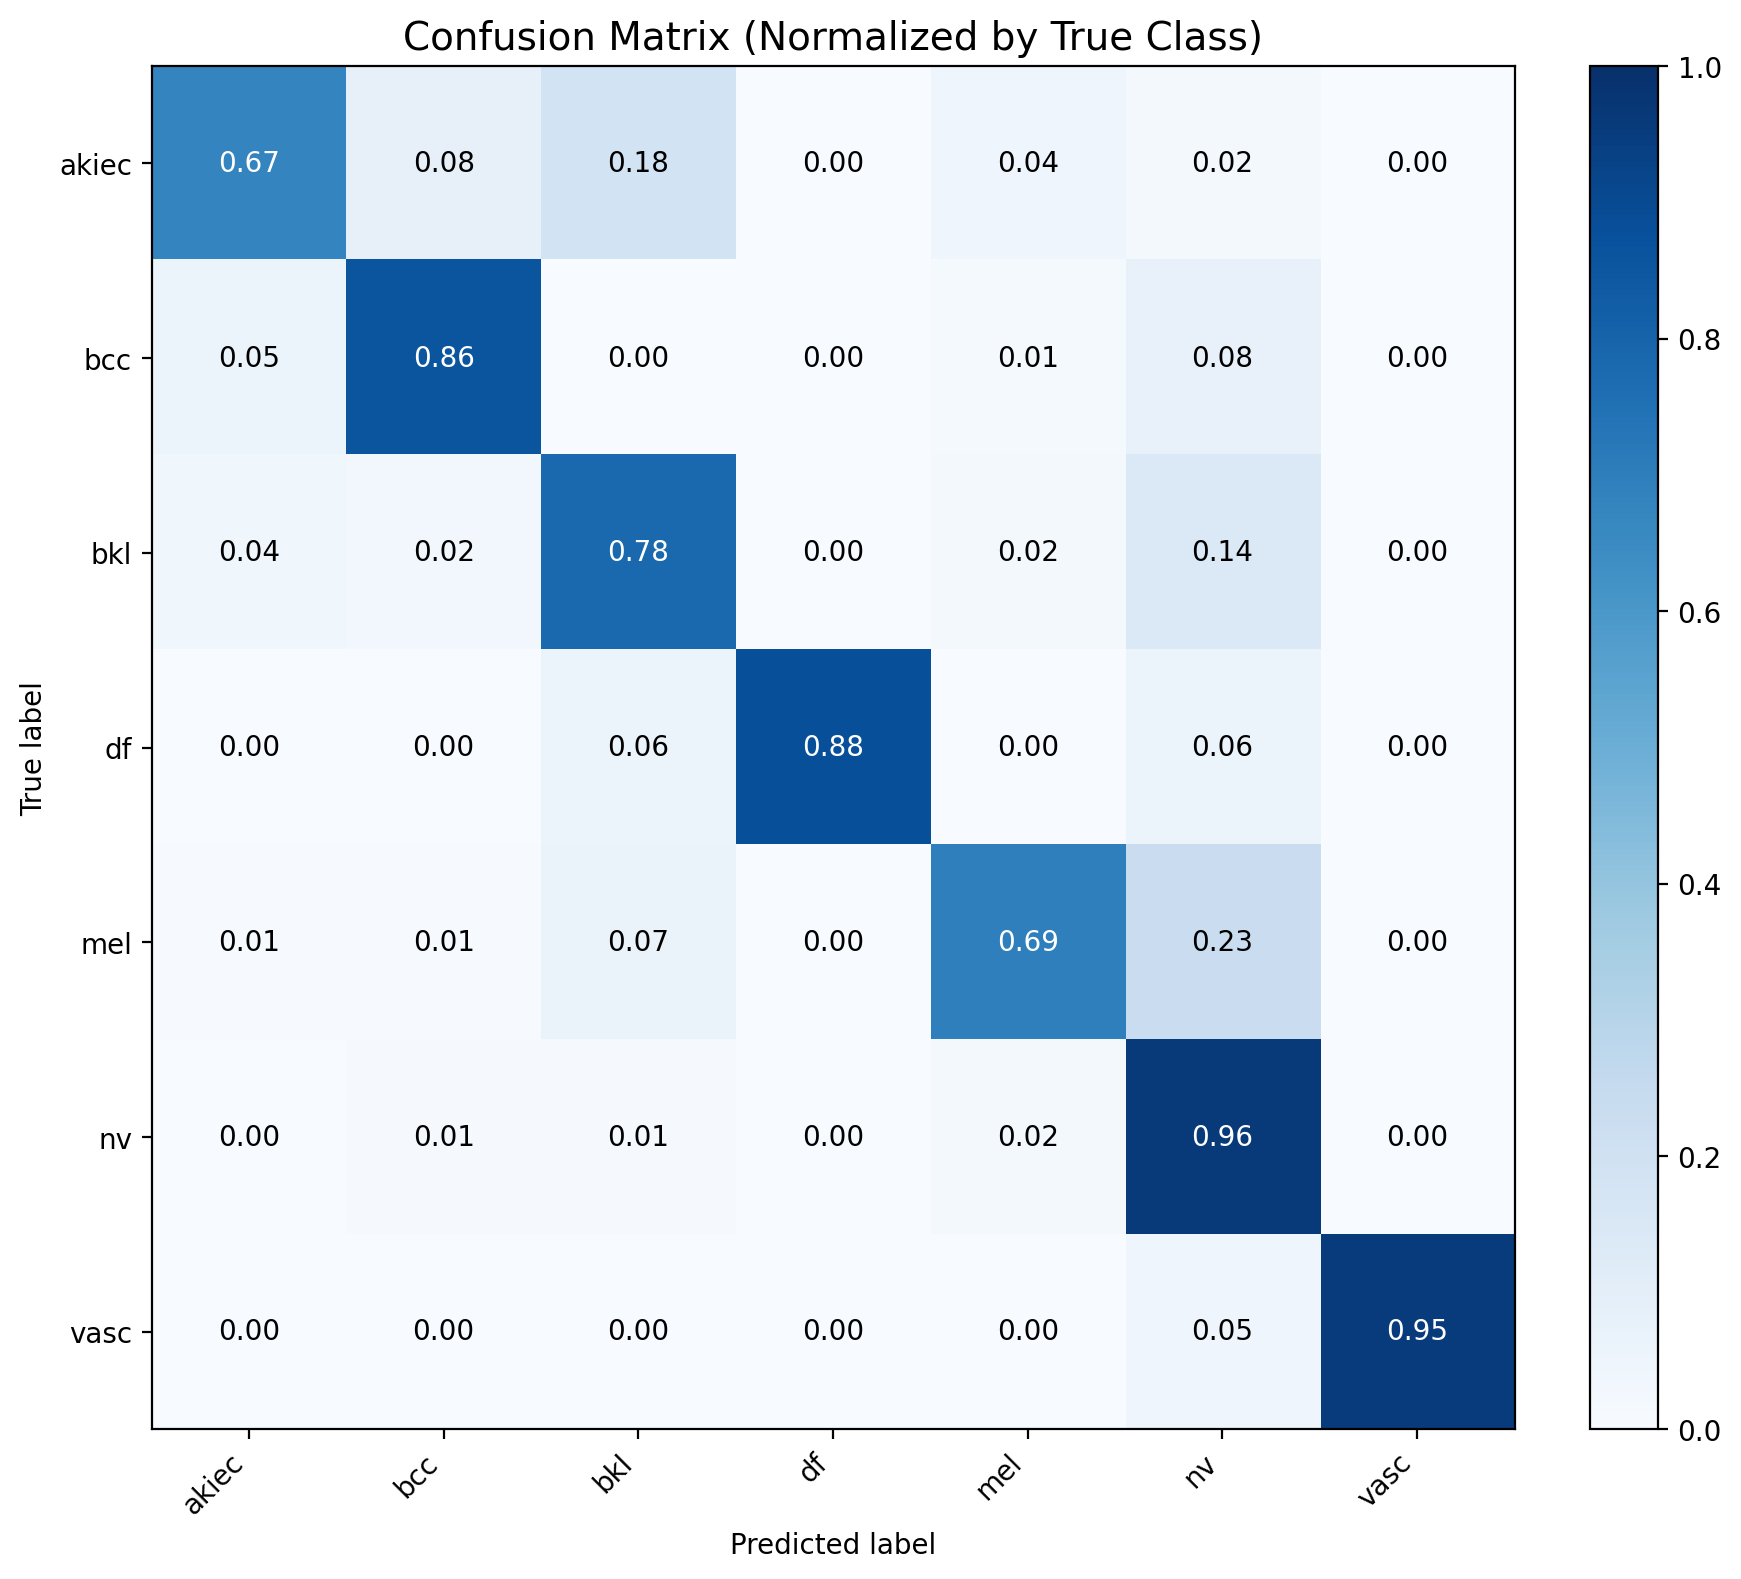
\includegraphics[width=0.65\textwidth]{thesis/figures/ensemble_confusion_matrix.png}
\end{center}

% ===================================================
\section{Code cho các biểu đồ trong report}
% ===================================================

\subsection{Confusion Matrix}

\begin{lstlisting}[caption={\texttt{src/utils/plots.py} --- vẽ confusion matrix}]
def _plot_single_confusion_matrix(cm_np, class_names, save_path, title,
                                   fmt='d', normalize=False):
    plt.figure(figsize=(10, 8))
    im = plt.imshow(cm_np, interpolation='nearest', cmap='Blues',
                    vmin=0, vmax=1 if normalize else None)
    plt.title(title, fontsize=14)
    plt.colorbar(im, fraction=0.046, pad=0.04)

    tick_marks = np.arange(len(class_names))
    plt.xticks(tick_marks, class_names, rotation=45, ha='right')
    plt.yticks(tick_marks, class_names)

    # Annotate từng ô với giá trị
    thresh = cm_np.max() / 2.0
    for i in range(cm_np.shape[0]):
        for j in range(cm_np.shape[1]):
            value = format(cm_np[i, j], fmt)
            plt.text(j, i, value, ha='center', va='center',
                     color='white' if cm_np[i, j] > thresh else 'black')

    plt.ylabel('True label'); plt.xlabel('Predicted label')
    plt.tight_layout(); plt.savefig(save_path, dpi=200); plt.close()


def plot_confusion_matrices(cm, class_names, raw_path, norm_path):
    cm_np = np.array(cm, dtype=np.int64)
    _plot_single_confusion_matrix(cm_np, class_names, raw_path,
                                   'Confusion Matrix (Raw Counts)', fmt='d')

    # Chuẩn hóa theo row (true class)
    row_sums = cm_np.sum(axis=1, keepdims=True)
    cm_norm = np.divide(cm_np, row_sums, where=row_sums != 0)
    _plot_single_confusion_matrix(cm_norm, class_names, norm_path,
        'Confusion Matrix (Normalized by True Class)', fmt='.2f',
        normalize=True)
\end{lstlisting}

\subsection{ROC Curves (One-vs-Rest)}

\begin{lstlisting}[caption={Vẽ ROC curves --- 1 đường cong cho mỗi lớp}]
def plot_roc_curves(roc_curves, save_path, title='ROC Curves (One-vs-Rest)'):
    colors = plt.cm.Set2(np.linspace(0, 1, len(roc_curves)))
    plt.figure(figsize=(9, 8))

    for i, (name, data) in enumerate(roc_curves.items()):
        fpr = data['fpr']; tpr = data['tpr']; auc_val = data['auc']
        plt.plot(fpr, tpr, color=colors[i], lw=2,
                 label=f'{name} (AUC = {auc_val:.3f})')

    plt.plot([0, 1], [0, 1], 'k--', lw=1, alpha=0.5,
             label='Random (AUC = 0.500)')
    plt.xlim([0, 1]); plt.ylim([0, 1.05])
    plt.xlabel('False Positive Rate'); plt.ylabel('True Positive Rate')
    plt.title(title); plt.legend(loc='lower right')
    plt.tight_layout(); plt.savefig(save_path, dpi=200); plt.close()
\end{lstlisting}

\subsection{Training History (loss, accuracy, F1, LR)}

\begin{lstlisting}[caption={Plot training history với 4 subplot}]
def plot_training_history_detailed(history, save_path):
    epochs = range(1, len(history['train_loss']) + 1)
    fig, axes = plt.subplots(1, 4, figsize=(24, 5))

    # (1) Loss
    axes[0].plot(epochs, history['train_loss'], 'o-', label='Train Loss')
    axes[0].plot(epochs, history['val_loss'],   's-', label='Val Loss')
    axes[0].set_title('Loss'); axes[0].legend(); axes[0].grid(alpha=0.3)

    # (2) Accuracy
    axes[1].plot(epochs, history['train_accuracy'], 'o-', label='Train Acc')
    axes[1].plot(epochs, history['val_accuracy'],   's-', label='Val Acc')
    axes[1].set_title('Accuracy'); axes[1].set_ylim(0, 1)

    # (3) Macro F1
    axes[2].plot(epochs, history['train_macro_f1'], 'o-', label='Train F1')
    axes[2].plot(epochs, history['val_macro_f1'],   's-', label='Val F1')
    axes[2].set_title('Macro F1'); axes[2].set_ylim(0, 1)

    # (4) Learning rate (cosine schedule)
    axes[3].plot(epochs, history['lr'], 'g-', lw=2)
    axes[3].set_title('Learning Rate Schedule')

    fig.suptitle('Training History', fontsize=14, fontweight='bold')
    plt.tight_layout(); plt.savefig(save_path, dpi=200); plt.close()
\end{lstlisting}

\subsection{Per-class F1 bar chart}

\begin{lstlisting}[caption={Per-class F1 + macro line}]
def plot_per_class_f1(per_class_f1, macro_f1, save_path):
    classes = list(per_class_f1.keys())
    values  = list(per_class_f1.values())
    colors  = ['#FF6B6B' if c in {'mel','bcc','akiec'} else '#4ECDC4'
               for c in classes]

    fig, ax = plt.subplots(figsize=(10, 5))
    bars = ax.bar(classes, values, color=colors, edgecolor='black')
    ax.axhline(macro_f1, color='red', linestyle='--', lw=2,
               label=f'Macro F1 = {macro_f1:.3f}')

    for bar, v in zip(bars, values):
        ax.text(bar.get_x() + bar.get_width()/2, v + 0.01,
                f'{v:.3f}', ha='center', fontweight='bold')

    ax.set_ylim(0, 1.05); ax.set_ylabel('F1 score')
    ax.set_title('Per-class F1 (red = malignant / pre-malignant)')
    ax.legend(); plt.tight_layout(); plt.savefig(save_path, dpi=200)
\end{lstlisting}

\subsection{Grad-CAM overlay}

\begin{lstlisting}[caption={Overlay heatmap lên ảnh gốc}]
@staticmethod
def overlay(original_image, heatmap, alpha=0.5, colormap=cv2.COLORMAP_JET):
    h, w = original_image.shape[:2]
    heatmap_resized = cv2.resize(heatmap, (w, h))
    heatmap_uint8   = np.uint8(255 * heatmap_resized)

    # Apply colormap (BGR) → convert to RGB
    colored_heatmap = cv2.applyColorMap(heatmap_uint8, colormap)
    colored_heatmap = cv2.cvtColor(colored_heatmap, cv2.COLOR_BGR2RGB)

    # Blend: alpha trên heatmap, (1-alpha) trên ảnh gốc
    overlay = (np.float32(colored_heatmap) * alpha +
               np.float32(original_image) * (1 - alpha))
    return np.clip(overlay, 0, 255).astype(np.uint8)
\end{lstlisting}

% ===================================================
\section{So sánh với State-of-the-Art}
% ===================================================

\begin{table}[h]
\centering\small
\begin{tabular}{lcccc}
\toprule
\textbf{Công trình} & \textbf{Năm} & \textbf{Phương pháp} & \textbf{Acc} & \textbf{Macro F1} \\
\midrule
Codella et al.        & 2018 & ResNet-152                   & 85.9 & 0.78 \\
Gessert et al.\ (winner) & 2018 & Ensemble EfficientNet + SENet & 88.5 & 0.82 \\
Mahbod et al.         & 2020 & Multi-scale CNN ensemble      & 88.7 & 0.83 \\
Pacheco \& Krohling   & 2020 & ResNet-50 + metadata fusion    & 89.0 & 0.83 \\
\rowcolor{usthblue!10}
\textbf{Đồ án này}    & 2026 & \textbf{4-model soft ensemble (n=5 hạt giống)} & \textbf{89.93 $\pm$ 0.66} & \textbf{0.852 $\pm$ 0.010} \\
\bottomrule
\end{tabular}
\end{table}

Đồ án đạt ngang hoặc \textit{nhỉnh hơn} các công trình SOTA \textbf{chỉ dùng ảnh} (không có metadata). Vượt qua khi có metadata bệnh nhân $\Rightarrow$ hướng phát triển tiếp theo.

% ===================================================
\section{Hạn chế và hướng phát triển}
% ===================================================

\subsection{Hạn chế}

\begin{itemize}[leftmargin=*]
  \item \textbf{Domain shift:} test cùng phân phối train (ISIC 2018), chưa kiểm chứng trên hospital khác.
  \item \textbf{Không metadata:} bỏ qua tuổi, giới, vị trí cơ thể.
  \item \textbf{Dataset 10K ảnh:} Swin overfit nhanh, ensemble nhạy với split.
  \item \textbf{Chỉ 7 lớp:} thực tế có hàng chục dạng tổn thương.
\end{itemize}

\subsection{Hướng phát triển}

\begin{enumerate}[leftmargin=*]
  \item \textbf{Multimodal:} kết hợp ảnh với metadata bệnh nhân.
  \item \textbf{Out-of-distribution evaluation:} test trên BCN20000, PAD-UFES-20.
  \item \textbf{Active learning:} cho bác sĩ chỉnh nhãn sai, định kỳ retrain.
  \item \textbf{Calibration sâu hơn:} temperature scaling, focal loss.
  \item \textbf{Edge deployment:} ONNX/TensorRT cho thiết bị dermoscopy di động.
\end{enumerate}

% ===================================================
\section{Tổng kết một trang}
% ===================================================

\textbf{Đồ án giải quyết vấn đề:} phân loại 7 lớp tổn thương da từ ảnh dermoscopy với độ chính xác và khả diễn giải đủ cho mục đích lâm sàng.

\textbf{Pipeline:} fine-tune 4 mô hình pretrained (EB0, RN50, DN121, Swin) trên ISIC 2018 với:
\begin{itemize}[leftmargin=*]
  \item \textbf{Stratified split} 70/15/15 giữ tỉ lệ 7 lớp.
  \item \textbf{Weighted Random Sampler} cân bằng mini-batch.
  \item \textbf{Mixup ($\alpha=0.2$) + CutMix ($\alpha=1.0$)} mỗi cái xác suất 0.5.
  \item \textbf{Label Smoothing} $\varepsilon = 0.1$.
  \item \textbf{AdamW} + cosine annealing + linear warmup.
  \item \textbf{Mixed precision} FP16.
\end{itemize}

\textbf{Ensemble} bằng soft voting (trung bình xác suất 4 mô hình) $\Rightarrow$ Accuracy 89.49\% / Macro F1 0.845 / AUC 0.980 ở hạt giống đại diện; trung bình qua 5 hạt giống ngẫu nhiên: $89{,}93 \pm 0{,}66\%$ / $0{,}852 \pm 0{,}010$ / $0{,}982 \pm 0{,}001$. McNemar test ($p < 10^{-7}$ vs.\ mô hình mạnh nhất) xác nhận ensemble vượt mọi mô hình đơn có ý nghĩa thống kê.

\textbf{Grad-CAM} cho heatmap giải thích quyết định mô hình; \texttt{focus\_ratio} > 0.6 chứng minh mô hình focus đúng tổn thương.

\textbf{Ablation} cho thấy Mixup/CutMix là thành phần quyết định nhất ($-4.51$\% F1 khi bỏ).

\textbf{Sản phẩm:} prototype Streamlit cho phép upload ảnh, nhận chẩn đoán + heatmap real-time.

\vspace{12pt}
\hrule
\vspace{6pt}
\begin{center}
\small \textit{Cẩm nang này là tài liệu học --- không thay thế thesis hoàn chỉnh, nhưng đủ để ôn thi và trả lời mọi câu hỏi cơ bản của hội đồng.}
\end{center}

\end{document}
